%Version 3.1 December 2024
% See section 11 of the User Manual for version history
%
%%%%%%%%%%%%%%%%%%%%%%%%%%%%%%%%%%%%%%%%%%%%%%%%%%%%%%%%%%%%%%%%%%%%%%
%%                                                                 %%
%% Please do not use \input{...} to include other tex files.       %%
%% Submit your LaTeX manuscript as one .tex document.              %%
%%                                                                 %%
%% All additional figures and files should be attached             %%
%% separately and not embedded in the \TeX\ document itself.       %%
%%                                                                 %%
%%%%%%%%%%%%%%%%%%%%%%%%%%%%%%%%%%%%%%%%%%%%%%%%%%%%%%%%%%%%%%%%%%%%%

%%\documentclass[referee,sn-basic]{sn-jnl}% referee option is meant for double line spacing

%%=======================================================%%
%% to print line numbers in the margin use lineno option %%
%%=======================================================%% 

%%\documentclass[lineno,pdflatex,sn-basic]{sn-jnl}% Basic Springer Nature Reference Style/Chemistry Reference Style

%%=========================================================================================%%
%% the documentclass is set to pdflatex as default. You can delete it if not appropriate.  %%
%%=========================================================================================%%

%%\documentclass[sn-basic]{sn-jnl}% Basic Springer Nature Reference Style/Chemistry Reference Style

%%Note: the following reference styles support Namedate and Numbered referencing. By default the style follows the most common style. To switch between the options you can add or remove “Numbered” in the optional parenthesis. 
%%The option is available for: sn-basic.bst, sn-chicago.bst%  
 
% \documentclass[pdflatex,sn-nature]{sn-jnl}% Style for submissions to Nature Portfolio journals
%%\documentclass[pdflatex,sn-basic]{sn-jnl}% Basic Springer Nature Reference Style/Chemistry Reference Style
\documentclass[pdflatex,sn-mathphys-num]{sn-jnl}% Math and Physical Sciences Numbered Reference Style
%%\documentclass[pdflatex,sn-mathphys-ay]{sn-jnl}% Math and Physical Sciences Author Year Reference Style
% \documentclass[pdflatex,sn-aps]{sn-jnl}% American Physical Society (APS) Reference Style
%%\documentclass[pdflatex,sn-vancouver-num]{sn-jnl}% Vancouver Numbered Reference Style
%%\documentclass[pdflatex,sn-vancouver-ay]{sn-jnl}% Vancouver Author Year Reference Style
%%\documentclass[pdflatex,sn-apa]{sn-jnl}% APA Reference Style
%%\documentclass[pdflatex,sn-chicago]{sn-jnl}% Chicago-based Humanities Reference Style

%%%% Standard Packages
%%<additional latex packages if required can be included here>

\usepackage{graphicx}%
\usepackage{multirow}%
\usepackage{amsmath,amssymb,amsfonts}%
\usepackage{amsthm}%
\usepackage{mathrsfs}%
\usepackage[title]{appendix}%
\usepackage{xcolor}%
\usepackage{textcomp}%
\usepackage{manyfoot}%
\usepackage{booktabs}%
\usepackage{algorithm}%
\usepackage{algorithmicx}%
\usepackage{algpseudocode}%
\usepackage{listings}%



%%%% Change Highlighting Packages (for reviewer responses)
\usepackage[markup=underlined,authormarkup=none]{changes}  % Main change tracking
\usepackage{soul}                                           % Text highlighting
\usepackage[normalem]{ulem}                                % Underlining and striking
\usepackage{todonotes}                                     % Marginal notes
\usepackage{xcolor}                                        % Extended colors (already included above)

% Configure change highlighting
\definecolor{addition}{RGB}{0,150,0}      % Green for additions
\definecolor{deletion}{RGB}{150,0,0}      % Red for deletions
\definecolor{highlight}{RGB}{255,255,0}   % Yellow for highlights
\definecolor{revision}{RGB}{0,0,150}      % Blue for revisions

% Define change author for tracking revisions
\definechangesauthor[name={Response to Reviewers}]{REV}

% Example usage (uncomment to use):
% \added{New text added in revision}
% \deleted{Old text removed in revision}
% \replaced{old text}{new text}
% \hl{yellow}{highlighted important text}
% \todo{This section was revised based on reviewer comments}


%%%% Change Highlighting Packages (for reviewer responses)
\usepackage[markup=underlined,authormarkup=none]{changes}  % Main change tracking
\usepackage{soul}                                           % Text highlighting
\usepackage[normalem]{ulem}                                % Underlining and striking
\usepackage{todonotes}                                     % Marginal notes
\usepackage{xcolor}                                        % Extended colors (already included above)

% Configure change highlighting
\definecolor{addition}{RGB}{0,150,0}      % Green for additions
\definecolor{deletion}{RGB}{150,0,0}      % Red for deletions
\definecolor{highlight}{RGB}{255,255,0}   % Yellow for highlights
\definecolor{revision}{RGB}{0,0,150}      % Blue for revisions

% Define change author for tracking revisions
\definechangesauthor[name={Response to Reviewers}]{REVISION}

% Examples you might use (all commented out):
% \added{New text added in revision}
% \deleted{Old text removed in revision}
% \replaced{old text}{new text}
% \hl{yellow}{highlighted important text}
% \hl{addition}{text highlighted in green}
% \hl{deletion}{text highlighted in red}
% \hl{revision}{text highlighted in blue}
% \sout{strikethrough text for deletions}
% \uwave{underwaved text for emphasis}
% \todo{This creates a marginal note}
% \todo[inline]{Inline todo note}
% \todo[color=red,size=\small]{Colored marginal note}
% \added[id=REVISION]{New text with author tracking}
% \deleted[id=REVISION]{Deleted text with author tracking}
% \replaced[id=REVISION]{old text}{new text with author tracking}
% \added[comment={Response to Reviewer 1}]{Text with comment}
% \highlight[color=orange]{Custom colored highlight}
% \todo[noline,color=green!40]{No line, colored note}


\usepackage{pgfplots}


\DeclareRobustCommand{\mathdefault}[1]{#1}

\usepackage{nicefrac}
\usepackage{xspace}

\newcommand{\vMLabel}{\textbf{vM}\xspace}
\newcommand{\EqJcLabel}{\textbf{Eq$\boldsymbol{J_c}$}\xspace}
\newcommand{\EqSigmaStarLabel}{\textbf{Eq$\boldsymbol{\sigma^*}$}\xspace}
\newcommand{\EqPiStarLabel}{\textbf{Eq$\boldsymbol{\Pi^*}$}\xspace}

%%%%

%%%%%=============================================================================%%%%
%%%%  Remarks: This template is provided to aid authors with the preparation
%%%%  of original research articles intended for submission to journals published 
%%%%  by Springer Nature. The guidance has been prepared in partnership with 
%%%%  production teams to conform to Springer Nature technical requirements. 
%%%%  Editorial and presentation requirements differ among journal portfolios and 
%%%%  research disciplines. You may find sections in this template are irrelevant 
%%%%  to your work and are empowered to omit any such section if allowed by the 
%%%%  journal you intend to submit to. The submission guidelines and policies 
%%%%  of the journal take precedence. A detailed User Manual is available in the 
%%%%  template package for technical guidance.
%%%%%=============================================================================%%%%

%% as per the requirement new theorem styles can be included as shown below
\theoremstyle{thmstyleone}%
\newtheorem{theorem}{Theorem}%  meant for continuous numbers
%%\newtheorem{theorem}{Theorem}[section]% meant for sectionwise numbers
%% optional argument [theorem] produces theorem numbering sequence instead of independent numbers for Proposition
\newtheorem{proposition}[theorem]{Proposition}% 
%%\newtheorem{proposition}{Proposition}% to get separate numbers for theorem and proposition etc.

\theoremstyle{thmstyletwo}%
\newtheorem{example}{Example}%
\newtheorem{remark}{Remark}%

\theoremstyle{thmstylethree}%
\newtheorem{definition}{Definition}%

\raggedbottom
%%\unnumbered% uncomment this for unnumbered level heads

\begin{document}

\title[Influence of material constitutive laws on the effective crack resistance of a simplified porous material in a numerical experiment]{\deleted{Influence of Material Constitutive Laws on Effective Crack Resistance in Heterogeneous Materials}\added{Influence of material constitutive laws on the effective crack resistance of a simplified porous material in a numerical experiment}}

%%=============================================================%%
%% GivenName	-> \fnm{Joergen W.}
%% Particle	-> \spfx{van der} -> surname prefix
%% FamilyName	-> \sur{Ploeg}
%% Suffix	-> \sfx{IV}
%% \author*[1,2]{\fnm{Joergen W.} \spfx{van der} \sur{Ploeg} 
%%  \sfx{IV}}\email{iauthor@gmail.com}
%%=============================================================%%

\author*[1]{\fnm{Alexander} \sur{Schl\"{u}ter}}
\email{alexander.schlueter@tu-darmstadt.de}

\author[1]{\fnm{Ronjit} \sur{Medda}}

\author[1]{\fnm{Ralf} \sur{M\"{u}ller}}

\affil*[1]{%
  \orgdiv{Institut f\"ur Mechanik, FB Bau- und Umweltingenieurwissenschaften},
  \orgname{TU Darmstadt},
  \orgaddress{%
    \street{Franziska-Braun-Stra{\ss}e 7},
    \city{Darmstadt},
    \postcode{64287},
    \country{Germany}
  }
}

%%==================================%%
%% Sample for unstructured abstract %%
%%==================================%%

\abstract{  
      In this work, we investigate the simulation-based determination of the effective fracture
resistance of porous materials while accounting for nonlinear, ductile material behavior.
Following the approach of Hossain et al.~\cite{hossain_effective_2014}, numerical experiments
with surfing boundary conditions are conducted to identify the effective crack resistance as
a macroscopic material parameter. Crack evolution in the microstructure is modeled using a
phase-field formulation without prescribing crack paths or growth continuity. The maximum
value of the macroscopically acting J-integral defines the driving force required for sustained
macroscopic crack advance and is taken as the effective fracture resistance. In contrast to
previous studies, a von~Mises plasticity model is employed to investigate ductile fracture in
porous metals. The results show that the effective fracture resistance is governed primarily
by the energy dissipation capacity of the material during crack renucleation at pores rather
than by tensile strength or microscopic fracture energy. A complementary three-dimensional
model confirms these findings, showing similar saturation behavior of the effective fracture
resistance with respect to microstructural wall width and good quantitative agreement with
the two-dimensional predictions.
}

%%================================%%
%% Sample for structured abstract %%
%%================================%%

% \abstract{\textbf{Purpose:} The abstract serves both as a general introduction to the topic and as a brief, non-technical summary of the main results and their implications. The abstract must not include subheadings (unless expressly permitted in the journal's Instructions to Authors), equations or citations. As a guide the abstract should not exceed 200 words. Most journals do not set a hard limit however authors are advised to check the author instructions for the journal they are submitting to.
% 
% \textbf{Methods:} The abstract serves both as a general introduction to the topic and as a brief, non-technical summary of the main results and their implications. The abstract must not include subheadings (unless expressly permitted in the journal's Instructions to Authors), equations or citations. As a guide the abstract should not exceed 200 words. Most journals do not set a hard limit however authors are advised to check the author instructions for the journal they are submitting to.
% 
% \textbf{Results:} The abstract serves both as a general introduction to the topic and as a brief, non-technical summary of the main results and their implications. The abstract must not include subheadings (unless expressly permitted in the journal's Instructions to Authors), equations or citations. As a guide the abstract should not exceed 200 words. Most journals do not set a hard limit however authors are advised to check the author instructions for the journal they are submitting to.
% 
% \textbf{Conclusion:} The abstract serves both as a general introduction to the topic and as a brief, non-technical summary of the main results and their implications. The abstract must not include subheadings (unless expressly permitted in the journal's Instructions to Authors), equations or citations. As a guide the abstract should not exceed 200 words. Most journals do not set a hard limit however authors are advised to check the author instructions for the journal they are submitting to.}

\keywords{Ductile Fracture, Porous Metals, Effective Fracture Toughness, Phase Field Model of Ductile Fracture, Numerical Experiment}

%%\pacs[JEL Classification]{D8, H51}

%%\pacs[MSC Classification]{35A01, 65L10, 65L12, 65L20, 65L70}

\maketitle

\section{Introduction}\label{sec:intro}

% Reviewer-style examples for the introduction (do not alter existing text):
\added{This sentence is a sample addition in the introduction.}
\deleted{This sentence is a sample deletion in the introduction.}
\replaced{This phrase is a sample replacement.}{This is the new phrase replacing the sample text.}

While homogenization techniques for elastic and plastic material properties are well established,
the homogenization of fracture toughness remains a comparatively young field of research.
Relevant quantities include the critical stress intensity factor \( K_{Ic} \),
appearing in Irwin’s criterion \( K_I = K_{Ic} \), and the critical energy release rate \( G_c \),
used in Griffith’s criterion \( G = G_c \).
Similarly,  more general fracture formulations based on the J-integral $J$ can be established, i.e.
\begin{equation}
    J = J_c,
    \label{eq:fracture_criterion_J}
\end{equation}
where \( J_c \) denotes the critical value of the J-integral and serves as a material parameter.
Such \deleted{criterions}\added{criteria}
remain applicable up to the onset of crack growth under monotonic loading even
in the presence of plasticity, as discussed in~\cite{gross_fracture_2011}.



A reliable determination of the fracture resistance parameters which are properties of the 
underlying material and microstructure is of significant
practical interest, particularly in light of the increasing use of
additive manufacturing technologies. For example, wire arc additive manufacturing (WAAM) enables the flexible combination of materials
and targeted microstructural design through the control of process parameters,
as demonstrated in~\cite{hauser_porosity_2021}. Fracture-mechanics-based criteria are often the appropriate tools
for strength assessment in these defect-rich materials.
However, their application requires material- and microstructure-dependent
fracture resistance parameters as mentioned above.

The existence of an effective fracture toughness for a given material
and the question of how it should be defined remain subjects
of active debate~\cite{lebihain_brittle_2021},
with several approaches proposed in the literature.
Schneider~\cite{schneider_fftbased_2020} suggests a variational definition that
relies on rigorous mathematical results for the homogenization of
the energy functional occurring in Bourdin's popular variational formulation of brittle fracture~\cite{bourdin_variational_2008}.
This idea is further pursued in~\cite{ernesti_fast_2021} and in
\cite{ernesti_computing_2022} for anisotropic fracture resistance.

Michel and Suquet~\cite{michel_merits_2022} propose the effective fracture
energy to be a directionally dependent quantity that corresponds to
the dissipated energy of the actual path of a crack through a suitable unit cell,
leading to full fracture of that unit cell in a given direction.
The authors also show that this definition yields a rigorous lower bound to the effective fracture energy.

In this work, we adopt the methodology introduced
by Hossain et al.~\cite{hossain_effective_2014} and further
developed and applied in~\cite{hsueh_stress_2018} for layered materials,
as well as considering anisotropy in~\cite{brach_anisotropy_2019},
to determine the effective fracture toughness of heterogeneous materials.

Their approach is based on a numerical experiment in which a representative material
region is subjected to boundary conditions that enforce complete separation.
The resulting microstructural crack evolution is
simulated using a phase-field model for fracture.
See, for example,~\cite{ambati_review_2015} for a comprehensive overview.
All of these contributions were limited to linear-elastic material behavior and two-dimensional problems.

Similarly, in previous studies by the authors of this contribution~\cite{schlueter_ermittlung_2025,schluter_determination_2025},
this framework was employed to determine the effective fracture toughness of porous materials,
assuming linear-elastic bulk behavior. For a simplified porous material, it was demonstrated that
the renucleation mechanism of cracks that are trapped in pores
determines the effective fracture toughness
and can act as a toughening factor if the pores are
spaced far enough apart. A saturation of the effective toughness was obtained above
a specific minimum distance between pores. This minimum distance depends on the
length at which cracks renucleate after being trapped, which among other factors also
depends on the pore shape.

As a first step in investigating the effective fracture toughness in ductile materials,
the effect of a non-linear elastic Ramberg--Osgood-type material law was also studied in~\cite{schluter_influence_2025}.
The results indicate that the energy dissipation capacity of the material law,
or the fracture resistance of the bulk material,
has a more critical influence on effective fracture resistance than the tensile strength.

In the present work, we aim to extend this analysis
toward additively manufactured metals, which typically exhibit pronounced ductile behavior.
In contrast to our previous work, which only considered reversible elastic material behavior,
albeit non-linear and consistent with von Mises plasticity under monotonic loading,
but which does not accurately capture unloading behavior,
we here also study the effect of true energy dissipation due to plasticity in ductile materials.
Since local unloading inevitably occurs during crack propagation,
even under monotonically increasing external loads,
this more closely matches true ductile fracture behavior.

In addition, we extend the approach of Hossain et al.~\cite{hossain_effective_2014} to take into account the three-dimensional
character of real porous materials with spherical pores.

This paper is structured as follows.
Section~\ref{sec:numericalExperiment} introduces the numerical experiment
proposed by Hossain et al.~\cite{hossain_effective_2014}.
Section~\ref{sec:phase_fiel_model_ductile} presents the phase-field
fracture formulation for both linear-elastic and von Mises-type plasticity material models.
Section~\ref{sec:2Dresults} focuses on the computation
of the effective fracture toughness for a simplified porous material
under two-dimensional plane strain assumptions
 using both constitutive descriptions.
Lastly, we extend the model to three dimensions and compare our findings for the von Mises-type plasticity model
for both the two-dimensional and three-dimensional cases.




\section{A Numerical Experiment to Determine the Effective Toughness
 of Materials with Complex Microstructure}
\label{sec:numericalExperiment}

% In this work, we limit ourselves to the description of brittle fracture and linear elastic materials. 

\begin{figure}[htb]
    \centering
    \resizebox{0.6\textwidth}{!}{\input{pics/num_experiment.pdf_t}}
    \caption{%
        Sketch of the numerical experiment introduced by Hossain et al.~\cite{hossain_effective_2014}. 
        Rather than conducting a macroscopic experiment, a region containing representative microstructural features is fractured in a numerical simulation while the energetic driving force required for fracture is measured.
    }
    \label{fig:numerical_experiment}
\end{figure}

The numerical experiment proposed by Hossain et al.~\cite{hossain_effective_2014} for the determination of an effective fracture toughness is conceptually closer to physical experiments than to the classical homogenization concepts commonly presented in micromechanics textbooks such as~\cite{gross_fracture_2011,nemat-nasser_micromechanics_2013}. 
The objective of this approach is the determination of an effective energetic fracture toughness\deleted{ $J_c^{\text{eff}}$, which}\added{, denoted by $J_c^{\text{eff}}$. This quantity} can subsequently be employed as a material parameter for predicting macroscopic crack growth according to the fracture criterion~(\ref{eq:fracture_criterion_J}).

The numerical experiment is structured as follows.
Instead of performing a physical experiment, a representative region\deleted{The term representative volume element is 
deliberately avoided, since the region no longer fulfills classical representativity requirements once fracture occurs, e.g. the 
separation of length scales.}\added{, rather than a representative volume element,}
 is selected that explicitly resolves the relevant microstructural features and whose fracture behavior is to be captured by \deleted{$J_c^{\text{eff}}$}\added{the effective energetic fracture toughness}.
\added{The term representative volume element is deliberately avoided because the region no longer fulfills classical representativity requirements once fracture occurs, e.g., the separation of length scales.}
This region is highlighted in dark gray in Fig.~\ref{fig:numerical_experiment}.
The corresponding length scale is referred to as the \textsl{microscale}, together with its associated \textsl{microstructure}.
The scale at which \deleted{$J_c^{\text{eff}}$}\added{this effective energetic fracture toughness} is applied is denoted as the \textsl{macroscale}.

The representative  region  is embedded within a surrounding matrix characterized by effective elastic properties, 
such as the effective Young's modulus $E^{\text{eff}}$ and Poisson's ratio $\nu^{\text{eff}}$ in the isotropic case.
This surrounding material facilitates the evaluation of surface integrals at the boundary and is shown in light gray in Fig.~\ref{fig:numerical_experiment}.
The union of the representative region and the surrounding matrix is considered as a continuum~$\Omega$. 
Macroscopic crack growth, corresponding to complete separation of the representative region along a prescribed direction, is enforced through appropriate boundary conditions.

In this work, only mode~I loading is considered.
Following the methodology of Hossain et al.~\cite{hossain_effective_2014}, so-called surfing boundary conditions are employed.
A fictitious macroscopic crack tip, illustrated by the black dot in Fig.~\ref{fig:numerical_experiment}, is propagated along a prescribed direction with velocity $\dot{x}_{\text{bc}}$, 
corresponding to the $x$-direction in the figure.
Displacements associated with mode~I crack opening are prescribed at the boundary using a fictitious 
stress intensity factor $K_I^{\text{bc}}$, namely
\begin{align}
    \begin{split}
        u_x &= \dfrac{K_I^{\text{bc}}}{2\mu_{\text{bc}}}  \sqrt{\dfrac{r}{2\pi}}\left(\kappa - \cos{\varphi}\right)\cos{\dfrac{\varphi}{2}},\\
        u_y &= \dfrac{K_I^{\text{bc}}}{2\mu_{\text{bc}}}  \sqrt{\dfrac{r}{2\pi}}\left(\kappa - \cos{\varphi}\right)\sin{\dfrac{\varphi}{2}},\\
        \text{where} \quad \kappa &= \dfrac{3 - \nu_{\text{bc}}}{1 + \nu_{\text{bc}}} \quad \text{and} \quad \mu_{\text{bc}} = \dfrac{E_{\text{bc}}}{2\left(1 + \nu_{\text{bc}}\right)}.
        \label{eq:surfing-bcs}
    \end{split}
\end{align}

Here, $r$ and $\varphi$ denote the polar coordinates of a system centered at the fictitious 
crack tip located at $x = \dot{x}_{\text{bc}} t$ and $y = 0$.
The boundary conditions are fully defined by the 
parameters $\dot{x}_{\text{bc}}$, $K_I^{\text{bc}}$ and the auxiliary fictitious material parameters  
$E_{\text{bc}}$, and $\nu_{\text{bc}}$.

The next step consists of simulating the evolution of the microscopic crack pattern until complete separation of the representative region is achieved.
The formulation must allow unrestricted crack evolution, since the interaction between microcracks and microstructural features governs the resulting fracture process, as indicated by the red crack paths in Fig.~\ref{fig:numerical_experiment}.
Furthermore, the simulation must be based on physically consistent principles.
An initial microscopic crack is introduced in this work and is depicted by the thick red line in Fig.~\ref{fig:numerical_experiment}.

Throughout the simulation, the macroscopically observable energetic driving force is evaluated at the boundary, indicated by the dashed blue contour in Fig.~\ref{fig:numerical_experiment}.
This quantity is computed in terms of the J-Integral
\begin{equation}
    J_x = \int_{\partial\Omega}\left(\psi_{\text{el}}(\boldsymbol{\varepsilon})\boldsymbol{1} - \left(\nabla\boldsymbol{u}\right)^T\boldsymbol{\sigma}\right)\boldsymbol{n} \, \mathrm{d}A \cdot \boldsymbol{e}_x,
    \label{eq:J-integral}
\end{equation}
where $\boldsymbol{e}_x$ denotes the unit vector in the macroscopic crack propagation direction.
The strain energy density is given by $\psi_{\text{el}}$, the linearized strain tensor\deleted{In this work, only small strain assumptions are considered. However, the framework could be extended to finite strains
in a straight forward manner.} by $\boldsymbol{\varepsilon} = \text{sym}(\nabla{\boldsymbol{u}})$, the displacement field by $\boldsymbol{u}$, the Cauchy stress by $\boldsymbol{\sigma}$, and the outward unit normal by $\boldsymbol{n}$.
\added{Only small strain assumptions are considered in this work.}

The effective fracture toughness is defined by Hossain et al.~\cite{hossain_effective_2014} as the maximum value attained by the J-Integral during the complete separation process,
\begin{equation}
    J_c^{\text{eff}} = \max(J_x) = J_x^{\text{max}}.
\end{equation}

The motivation for this definition is that loading levels below $J_x^{\text{max}}$ lead to crack arrest within the simulation and 
therefore do not result in macroscopic crack propagation, 
understood as full separation of the representative region.

The insensitivity of $J_x^{\text{max}}$ with respect to the precise implementation of boundary conditions has been demonstrated in previous studies such as~\cite{hossain_effective_2014, bohnen_simulation_2024}.
Independence from the initial microscopic crack configuration and adequate representation of fracture mechanisms can be ensured by selecting a sufficiently large representative region that contains an appropriate number of microstructural features\deleted{This presumes a sufficiently homogeneous spatial distribution of microstructural features, analogous to assumptions made for representative volume elements in micromechanics.}.
\added{This presumes a sufficiently homogeneous spatial distribution of microstructural features, analogous to assumptions made for representative volume elements in micromechanics.}


\section{A phase field model of ductile fracture}\label{sec:phase_fiel_model_ductile}

In order to model fracture in ductile materials under quasi-static loading conditions, we employ the model proposed in~\cite{noll_3d_2020}. 
The constitutive behavior of the considered continuum $\Omega$ with boundary $\partial\Omega$ in the unfractured state is described by von Mises plasticity with isotropic linear hardening. 
Small deformation theory is assumed to be sufficient.

In this case, the total linearized strain
\begin{equation}
    \boldsymbol{\varepsilon} = \dfrac{1}{2}\left(\nabla{\boldsymbol{u}} + \nabla{\boldsymbol{u}}^T\right)
\end{equation}
with $\boldsymbol{u}$ denoting the displacement field can be decomposed into a reversible elastic strain $\boldsymbol{\varepsilon}^e$ caused by the current stress $\boldsymbol{\sigma}$ and a plastic strain $\boldsymbol{\varepsilon}^p$ that remains after complete unloading as
\begin{equation}
  \boldsymbol{\varepsilon} =  \boldsymbol{\varepsilon}^e + \boldsymbol{\varepsilon}^p.
\end{equation}

To model linear isotropic strain hardening, a scalar internal state variable $\alpha$ is introduced that is related to the density of dislocations in the crystallographic microstructure. 
The yield stress is postulated as
\begin{equation}
    \sigma_Y(\alpha) = \sigma_y + H\alpha
\end{equation}
with $H$ denoting the hardening modulus and $\sigma_y$ the initial yield stress. 
Plastic deformation is assumed to be driven exclusively by the deviatoric part of the stress state, which is typical for metals. 
Accordingly, a $J_2$ yield function is introduced as
\begin{equation}
    f(\boldsymbol{\sigma},\alpha) = \|\boldsymbol{s}\| - \sqrt{\dfrac{2}{3}}\left(\sigma_y+H\alpha\right), 
    \quad \text{with} \quad 
    \boldsymbol{s} = \text{dev}\left(\boldsymbol{\sigma}\right) = \boldsymbol{\sigma}-\dfrac{1}{3}\text{tr}\left(\boldsymbol{\sigma}\right)\boldsymbol{1},
\end{equation}
where $\text{tr}(*)$ denotes the trace operator and $\boldsymbol{1}$ is the second order identity tensor.
The yield function $f$ determines the onset of plastic flow through the condition
\begin{equation}
    f(\boldsymbol{\sigma},\alpha) = 0 \quad \text{if yielding occurs}.
\end{equation}

Consistent with the principle of maximum dissipation, the evolution equations of the plastic variables are given by
\begin{equation}
    \dot{\boldsymbol{\varepsilon}}^p = \dot{\gamma}\boldsymbol{N},
    \label{eq:evolution_eps_p}
\end{equation}
and
\begin{equation}
    \dot{\alpha} = \sqrt{\dfrac{2}{3}}\,\dot{\gamma},
    \label{eq:evolution_alpha}
\end{equation}
where
\begin{equation}
    \boldsymbol{N} = \dfrac{\boldsymbol{s}}{\|\boldsymbol{s}\|}.
\end{equation}
In addition, the Karush--Kuhn--Tucker conditions
\begin{equation}
    f(\boldsymbol{\sigma},\alpha) \le 0, 
    \quad \dot{\gamma} \ge 0, 
    \quad f\,\dot{\gamma} = 0
\end{equation}
must be satisfied to ensure a physically consistent description of plasticity.

To model fracture, an additional field variable $s(\boldsymbol{x},t) \in [0,1]$ is introduced. 
The value $s=0$ corresponds to fully fractured material, while $s=1$ represents intact material sufficiently far from cracks. 
In the transition region, the field varies smoothly between these two values, providing a diffuse representation of cracks in a continuum setting.

Using this phase field variable, the total energy of the continuum $\Omega$ is given by
\begin{equation}
    E_{\rm{ep}} = \int_{\Omega} \left[ 
    \psi_{\rm{el}}(\boldsymbol{\varepsilon},\boldsymbol{\varepsilon}^p,s) 
    + \psi_{\rm{fr}}(s,\nabla{s}) 
    + \psi_{\rm{pl}}(\alpha,s)
    \right] \, \mathrm{d}V,
\end{equation}
where
\begin{equation}
    \psi_{\rm{el}}(\boldsymbol{\varepsilon},\boldsymbol{\varepsilon}^p,s)
    = g(s)\,w_{\rm{el}}(\boldsymbol{\varepsilon},\boldsymbol{\varepsilon}^p)
    = g(s)\dfrac{1}{2}
    \left(\boldsymbol{\varepsilon}-\boldsymbol{\varepsilon}^p\right)
    {:}
    \left(\boldsymbol{\mathbb{C}}{:}
    \left(\boldsymbol{\varepsilon}-\boldsymbol{\varepsilon}^p\right)\right).
\end{equation}
Here, $\boldsymbol{\mathbb{C}}$ denotes the elastic stiffness tensor, which is degraded in the presence of cracks through the degradation function
\begin{equation}
    g(s) = \beta\left(s^3 - s^2\right) + 3s^2 - 2s^3 + \eta,
    \label{eq:deg_grad}
\end{equation}
with $\beta = 0.2$ controlling the slope of $g(s)$ at $s=1$, and $\eta = 10^{-5}$ serving as a residual stiffness parameter to avoid ill-conditioned tangents when solving the problem using a Newton scheme.

To account for crack driving forces arising from the accumulation of plastic deformation, as expected for ductile fracture, the plastic contribution to the energy is also degraded according to
\begin{equation}
    \psi_{\rm{pl}}(\alpha,s) = g(s)\left(\dfrac{1}{2}H\alpha^2 + \sigma_y\alpha\right).
\end{equation}

Finally, the fracture energy contribution is given by
\begin{equation}
    \psi_{\rm{fr}} = J_c
    \underbrace{\left(
    \dfrac{(1-s)^2}{2\epsilon} + 2\epsilon\|\nabla{s}\|^2
    \right)}_{\bar{A}},
\end{equation}
which represents the energy dissipated due to fracture. 
Here, $\bar{A}$ approximates the crack surface, $J_c$ denotes the material-specific fracture energy per unit crack surface area, and $\epsilon$ controls the width of the diffuse crack zone.

For the linear elastic case, it can be shown that the zero set of $s$ minimizing the total energy converges to minimizers obtained with a sharp crack representation as $\epsilon \to 0$, see~\cite{chambolle_approximation_2004}.

A thermodynamically consistent evolution equation for the phase field variable $s$, governing crack growth, is derived using a variant of the Coleman--Noll procedure as described in~\cite{noll_3d_2020},
\begin{align}
    \begin{split}
    \dot{s} = -M \Bigg[
    g'(s)\left(\psi_{\rm{el}} + \left(\sigma_y+\dfrac{1}{2}H\alpha\right)\alpha\right)
    - J_c\left(2\epsilon\Delta{s} + \dfrac{1-s}{2\epsilon}\right)
    \Bigg]
    \quad \text{in} \ \Omega, \\
    \nabla{s}\cdot{\boldsymbol{n}} = 0 \quad \text{on} \ \partial\Omega.
    \label{eq:evolution_s}
    \end{split}
\end{align}

The mobility parameter $M$ arises from the introduction of a viscous regularization and facilitates the numerical solution of fracture problems under quasi-static loading conditions. 
Accordingly, static equilibrium is assumed in the form
\begin{equation}
    \text{div}(\boldsymbol{\sigma}) = \boldsymbol{0} \quad \text{in} \ \Omega, 
    \quad 
    \boldsymbol{\sigma}\boldsymbol{n} = \boldsymbol{t}^* 
    \quad \text{on} \ \partial\Omega_t,
    \label{eq:equilibrium}
\end{equation}
where the stress tensor $\boldsymbol{\sigma}$ is computed under the assumption of isotropic linear elasticity as
\begin{equation}
    \boldsymbol{\sigma} = g(s)\left[
    K\,\text{tr}(\boldsymbol{\varepsilon})\,\boldsymbol{1}
    + 2\mu\left(\text{dev}(\boldsymbol{\varepsilon}) - \boldsymbol{\varepsilon}^p\right)
    \right].
    \label{eq:sigma_plast}
\end{equation}

The evolution equations for the primary fields $\boldsymbol{u}$ and $s$, together with the evolution equations for the plastic variables and the Karush--Kuhn--Tucker conditions, define the coupled phase field formulation for ductile fracture.


\subsection{A phase field model for brittle fracture}
\label{sec:phasefield_elastic}

In order to judge the influence of ductile material behavior on the effective fracture toughness, 
we also consider a phase field model of brittle fracture that assumes linear elastic material behavior. 
Details of this model are\deleted{ e.g. described in ~\cite{kuhn_continuum_2010}}\added{ described, e.g., by~\cite{kuhn_continuum_2010}}. The governing equations 
are very similar to (\ref{eq:evolution_s}) and (\ref{eq:equilibrium}) but don't have
any contributions of the plastic variables  

\begin{equation}
    \dot{s} = -M \left[g'(s)\psi_{\rm{el}}  - J_c\left(2\epsilon\Delta{s} + \dfrac{1-s}{2\epsilon}\right)\right] \quad \text{in} \, \Omega, \quad \nabla{s}\cdot{\boldsymbol{n}} = 0\quad\text{on}\,\partial\Omega,
    \label{eq:evolution_s_elastic}
\end{equation}

\begin{equation}
    \text{div}(\boldsymbol{\sigma}) = \boldsymbol{0} \quad \text{in} \, \Omega, \quad{\boldsymbol{\sigma} \boldsymbol{n} =\boldsymbol{t}^*} \quad\text{on}\,\partial\Omega_t
    \label{eq:equilibrium_elastic}
\end{equation}

with 

\begin{equation}
    \boldsymbol{\sigma} = g(s)\left[K \text{tr}\boldsymbol{\varepsilon}\boldsymbol{1} + 2\mu\text{dev}(\boldsymbol{\varepsilon})\right].
\end{equation}


% The origins of phase field models like the one presented in the previous section can be found in the original Griffith-criterion, which states that cracks can grow if the energy released by crack growth is equal to the energy required to create the new crack surface which is a material parameter. 

\subsection{Parameter sets}
\label{sec:parameter_sets}
In the following chapters, the influence of the material law and various parameters on the fracture behavior of the phase field model,
as well as on the effective fracture resistance of a porous material, is investigated.
To isolate the impact of individual parameters, three specific parameter sets are studied.
These are defined for a given reference fracture resistance $J_c^0$, Lam\'{e} parameter $\mu_0$, and length scale $L$ as: 
\begin{itemize}
\setlength{\itemindent}{4em}


\item[\textbf{vM}:]
\parbox[t]{\dimexpr\linewidth-4em\relax}{
the von Mises-type plasticity model of section~\ref{sec:phase_fiel_model_ductile},
with $\sigma_y=1.0\sqrt{\nicefrac{J_c^0\mu_0}{L}}$, $H=0.22\mu_0$,
$\lambda=\mu_0$ and $J_c=1.0J_c^0$,
}

\item[\textbf{Eq$\boldsymbol{J_c}$}:]
\parbox[t]{\dimexpr\linewidth-4em\relax}{
the linear elastic model of section~\ref{sec:phasefield_elastic}
with $J_c=1.0J_c^0$ and $\lambda=\mu_0$,
}

\item[\textbf{Eq$\boldsymbol{\sigma^*}$}:]
\parbox[t]{\dimexpr\linewidth-4em\relax}{
the linear elastic model of section~\ref{sec:phasefield_elastic}
with fracture resistance $J_c=0.5679J_c^0$ and $\lambda=\mu_0$.
}
\end{itemize}


\subsection{Relation to an Energetic Fracture Criterion}
\label{sec:steady_growth_griffith}

\begin{figure}[htb]
    \centering
    \resizebox{0.8\textwidth}{!}{\includegraphics[]{pics/griffith_deformed.png}}
    \vspace{0.2cm}
    \caption{%
        Deformed contour plot of the phase field $s$ in a strip of size $16L \times 2L$ for the simulation \textbf{Eq$\boldsymbol{J_c}$}. The deformation is scaled by a factor of 0.3. 
    }
    \label{fig:griffith_deformed}
\begin{picture}(0,0)
    \put(133,86){$x$}
    \put(-155,136){$y$}
    \put(3,68){$s$}
\end{picture}    
\end{figure}

\begin{figure}[htb]
    \centering
    \includegraphics[width=0.8\textwidth]{pics/PAPER_01_all_Jx_vs_xct_pf__vM.png}
    \caption{%
        J-Integral versus crack tip position $x_{ct}$ measured during a simulation of crack propagation in a homogeneous material strip of size $16L \times 2L$.
    }
    \label{fig:PAPER_01_all_Jx_vs_xct_pf_2}
\end{figure}

\begin{figure}[htb]
    \centering
    \resizebox{0.95\textwidth}{!}{\includegraphics{pics/alpha_t_6.2495.png}}
    \vspace{0.2cm}
    \caption{%
        Plastic variable $\alpha$ at $t=6.25\nicefrac{L}{\dot{x}_{\rm bc}}$ for the simulation with the 
        \vMLabel data set.
    }
    \label{fig:plasticity_vm_jeff}

    \begin{picture}(0,0)
        \put(-50,25){%
            \resizebox{0.25\textwidth}{!}{\includegraphics{pics/legend_alpha.png}}
        }
        \put(-5,55){$\alpha$}
    \end{picture}
\end{figure}

In order to highlight the connection of the presented phase field model to the fracture criterion~(\ref{eq:fracture_criterion_J}), a simulation was performed in which crack growth was enforced using the surfing boundary conditions described in section~\ref{sec:numericalExperiment}. The computational domain consisted of a $16L \times 2L$ strip of homogeneous material with the following parameters: $\lambda_0 = \mu_0$, $M = 1000.0 \nicefrac{\dot{x}_{\text{bc}}}{J_c^0}$, $\epsilon = 0.1L$, and element edge length $\Delta{h} = 0.02L$. The boundary condition parameters were $\nu_{\text{bc}} = 0.25$, $E_{\text{bc}} = 2.5\mu_{0}$, and $K_I^{\text{bc}} = \sqrt{J_c^0 \cdot 2.5\mu_{0}}$, which enforce crack propagation in the $x$-direction, as shown in Fig.~\ref{fig:griffith_deformed}.

These simulations were conducted using the three parameter sets introduced in section~\ref{sec:parameter_sets}. 
As discussed in section~\ref{sec:numericalExperiment}, the J-Integral~(\ref{eq:J-integral}) evaluated at the boundary of the domain quantifies the energetic driving force for crack propagation. 
The results show that the J-Integral remains nearly constant throughout the crack propagation process, as illustrated in Fig.~\ref{fig:PAPER_01_all_Jx_vs_xct_pf_2}.

As established in the literature~\cite{tanne_crack_2018}, the actual numerical fracture resistance $J_c^{\text{num}}$ obtained from finite element simulations is typically higher than the specified parameter $J_c$. For a given material law, this deviation primarily depends on the ratio $\nicefrac{\Delta{h}}{\epsilon}$, see also~\cite{tanne_crack_2018}. In the current setup, the following approximate values were observed:
\begin{itemize}
    \item $J_c^{\text{num}} \approx 1.50J_c^0$ for the von Mises material model \vMLabel,
    \item $J_c^{\text{num}} \approx 1.12J_c^0$ for \EqJcLabel,
    \item $J_c^{\text{num}} \approx 0.64J_c^0$ for \EqSigmaStarLabel,
\end{itemize}
It is worth noting that the von Mises material model yields a significantly higher numerical fracture resistance than the linear elastic model at the same specified $J_c$. The evolution of plastic variables remains largely limited to the crack path, as can be observed in Fig.~\ref{fig:plasticity_vm_jeff}, so that the linear elastic formulation of the J-Integral (\ref{eq:J-integral}) remains a good approximation even in the presence of plasticity. However, the ductile material law still has a significant effect on the crack driving force. In general, the larger the fracture resistance $J_c$, the higher the required crack driving force $J_x$ must be to sustain steady crack growth.

These simulations confirm that pre-existing cracks propagate according to an energetic criterion equivalent to \added{the criterion in Eq.~}\deleted{~}(\ref{eq:fracture_criterion_J}): a crack advances when the energetic driving force equals the fracture resistance. Throughout this work, such behavior is referred to as energetically driven crack growth. A reference numerical energetic fracture resistance is defined as the value obtained from parameter set \EqJcLabel:
\begin{equation}
    J_c^{\text{num}} \approx 1.12J_c.
\end{equation}

\subsection{Stress driven crack nucleation}

\begin{figure}[htb]
    \centering
    \resizebox{0.7\textwidth}{!}{\includegraphics[]{pics/1D_bar.png}}
    \caption{%
       One-dimensional bar subjected to a displacement load $u_0$.
    } 
    \label{fig:setup_crack_nucleation}
\end{figure}

\begin{figure}[htb]
    \centering
    \begin{minipage}[t]{0.49\textwidth}
        \centering
        \resizebox{\linewidth}{!}{%
            \input{pics/PAPER_reaction_forces_1D_EQ_ONLY.pgf}%
        }
        \caption{Stress $\sigma$ vs.\ strain $\varepsilon$. The dots indicate the fracture stress $\sigma^*$, whereas the vertical dashed lines display the fracture strain $\varepsilon^*$.}
        \label{fig:reaction_forces}
    \end{minipage}%
    \hfill
    \begin{minipage}[t]{0.49\textwidth}
        \centering
        \resizebox{\linewidth}{!}{%
            \input{pics/PAPER_energy_vs_displacement_1D_EQ_ONLY.pgf}%
        }
        \caption{Energy $\Pi$ vs.\ applied displacement.}
        \label{fig:energy_vs_displacement}
    \end{minipage}
\end{figure}

In addition to satisfying the fracture criterion~(\ref{eq:fracture_criterion_J}) for pre-existing cracks, crack nucleation in previously undamaged material can also be predicted using phase-field models.

In the one-dimensional linear elastic case with the cubic degradation function~(\ref{eq:deg_grad}) and $\beta = 0$, it can be shown analytically that crack nucleation occurs once the stress level reaches a critical value slightly below
\begin{equation}
    \sigma_c = \dfrac{81}{50}\sqrt{\dfrac{2\mu J_c}{15.0\epsilon}},
    \label{eq:sig_c}
\end{equation}
see~\cite{schlueter_phase_2018}. For the ductile phase-field fracture model, also employing the cubic degradation function~(\ref{eq:deg_grad}) with $\beta = 0$, the critical strain is given by
\begin{equation}
    \varepsilon_c = \sqrt{\dfrac{1}{3} \dfrac{E+H}{EH}
    \left[\left(\dfrac{\sigma_y^2}{H} + \dfrac{5}{18}\dfrac{J_c}{\epsilon}\right)
    + \sqrt{4\left(\dfrac{\sigma_y^2}{H}\right)^2
    + \dfrac{8}{9} \dfrac{\sigma_y^2 J_c}{H\epsilon}
    + \dfrac{25}{324} \left(\dfrac{J_c}{\epsilon}\right)^2}\,\right]},
    \label{eq:ductile_fracture_strain}
\end{equation}
for $E = 2\mu_0$, and the corresponding critical stress then follows from~(\ref{eq:sigma_plast}), cf.~\cite{noll_3d_2020}. Strictly speaking, these relations hold only in one dimension, but they provide good estimates for two- and three-dimensional scenarios, where cracks tend to form spontaneously once a stress level close to $\sigma_c$ is exceeded in a sufficiently large region—typically on the order of several multiples of $\epsilon$, cf.~\cite{kuhn_numerical_2013}. Due to the relevance of this stress threshold, this mechanism is referred to as \textsl{stress-driven crack nucleation}, in contrast to the \textsl{energetically driven crack growth} mechanism discussed previously.

Stress-driven crack nucleation is demonstrated using the one-dimensional setup shown in Fig.~\ref{fig:setup_crack_nucleation}. The domain consists of an initially undamaged bar (i.e., $s = 1$ everywhere) of length $2L$, subjected to a linearly increasing displacement load $u_0$ applied at both ends. The field equations are reduced to one dimension by setting $\lambda = 0$, $u_y = 0$, and $u_z = 0$. The material parameters are $\mu_0$, $M = 1000.0\,\nicefrac{\dot{x}_{\text{bc}}}{J_c^0}$, $\epsilon = 0.1L$, and an element edge length of $\Delta h = 0.01L$.

Simulations were conducted for the three parameter sets introduced in Section~\ref{sec:parameter_sets}. To intentionally trigger crack nucleation at $x = 0$, the fracture toughness $J_c$ was locally reduced by 1\% \deleted{in the region $-3\Delta h \le x \le 3\Delta h$}\added{within a region extending from $x=-3\Delta h$ to $x=3\Delta h$}.

In all cases, fracture was observed to occur at $x = 0$ once a critical load level was 
reached. For the same energetic fracture resistance $J_c$, the linear elastic model with parameters \EqJcLabel yielded a significantly higher fracture stress of $\sigma^* = 1.72\sigma_y$ than the von~Mises-type model \vMLabel, which resulted in $\sigma^* = 1.31\sigma_y$. However, the fracture strain was smaller in the linear elastic case, with $\varepsilon^* \approx 1.08\sqrt{\nicefrac{J_c^0}{\mu_0 L}}$ for \EqJcLabel compared to $\varepsilon^* \approx 1.18\sqrt{\nicefrac{J_c^0}{\mu_0 L}}$ for \vMLabel, as shown in Fig.~\ref{fig:reaction_forces}.

To match the fracture stress of the von~Mises model in a linear elastic simulation, the fracture resistance was reduced to $J_c = 0.5679J_c^0$ in \EqSigmaStarLabel. This adjustment resulted in an almost equivalent fracture stress of $\sigma^* = 1.30\sigma_y$ compared to the von~Mises model, but a significantly lower fracture strain of only $\varepsilon^* \approx 0.82\sqrt{\nicefrac{J_c^0}{\mu_0 L}}$.

The elastic energy dissipated due to fracture is defined as
\begin{equation}
   \Pi(\varepsilon) = \int_{-L}^{L}
   \left[\int_{0}^{\varepsilon} \boldsymbol{\sigma} :
   \mathrm{d}\tilde{\boldsymbol{\varepsilon}}\right] \mathrm{d}x,
   \label{eq:total_energy}
\end{equation}
and is evaluated at the fracture strain $\varepsilon = \varepsilon^*$. The evolution of this energy for all three simulations is shown in Fig.~\ref{fig:energy_vs_displacement}. The highest dissipated energy is observed in the linear elastic simulation \EqJcLabel, with $\Pi^* \approx 2.22J_c^0 L$, followed by the von~Mises simulation \vMLabel with $\Pi^* \approx 2.16J_c^0 L$. In contrast, the linear elastic simulation \EqSigmaStarLabel dissipates only $\Pi^* \approx 1.29J_c^0 L$.





\section{Effective Toughness of a Simplified 2D Porous Material}
\label{sec:2Dresults}



\begin{figure}[htb]
    \centering
    \resizebox{0.9\textwidth}{!}{\includegraphics[]{pics/setup.png}}
    \vspace{10mm}
    \caption{%
        a) Simulation domain for the numerical experiment for $w_s = 1.0L$. Red indicates regions with bulk material stiffness, whereas blue shows regions with effective stiffness.
        b) Typical crack pattern.
        c) Employed triangular finite element mesh.
    }
    \label{fig:setup_crack_growth}
    \begin{picture}(0,0)
        \put(-173,207){$y$}
        \put(-63,136){$x$}
        \put(-180,60){a)}
        \put(-59,60){b)}
        \put(62,60){c)}
    \end{picture}
\end{figure}

\begin{figure}[htb]
    \centering
    \resizebox{0.4\textwidth}{!}{\input{pics/PAPER_00_xct_pf_vs_xct_KI_vonMises.pgf}}
    \caption{%
        Position of the surfing boundary conditions $x_{\text{bc}}$ and the crack tip position $x_{\text{ct}}$.
    }
    \label{fig:PAPER_00_xct_pf_vs_xct_KI_diamond}
\end{figure}

\begin{figure}[htb]
    \centering
    \includegraphics[width=0.8\textwidth]{pics/PAPER_clean_Jx_vs_xct_SIG_Jc_vonMises.png}
    \caption{%
        J-Integral vs.\ crack tip position $x_{ct}$ for $w_s = 1.0L$.
    }
    \begin{picture}(0,0)
        \put(-89,70){\includegraphics[width=0.425\textwidth]{pics/holes_s_middle_row.png}}
    \end{picture}
    \label{fig:PAPER_02_all_Jx_vs_xct_pf_diamond_holes}
\end{figure}


\begin{figure}[htb]
    \centering
    \begin{minipage}{0.49\textwidth}
        \centering
        \resizebox{\textwidth}{!}{\includegraphics[width=\textwidth]{pics/PAPER_04_Jx_vs_xct_all_vonMises.png}}
        \caption{Section of the J-Integral $J_x$ vs.\ crack tip position $x_{ct}$ between pores two and four for the parameter set \vMLabel and varying $w_s$.}
        \label{fig:PAPER_04_Jx_vs_xct_all_von_Mises}
    \end{minipage}
    \hfill
    \begin{minipage}{0.49\textwidth}
        \centering
        \includegraphics[width=\textwidth]{pics/PAPER_03A_Jx_vs_xct_all_linear_elastic_gc10.png}
        \caption{Section of the J-Integral $J_x$ vs.\ crack tip position $x_{ct}$ between pores two and four for the parameter set \textbf{Eq}$\boldsymbol{J_c}$ and varying $w_s$.}
        \label{fig:PAPER_03A_Jx_vs_xct_all_linear_elastic_gc10}
    \end{minipage}

    \vspace{3mm}

    \begin{minipage}{0.49\textwidth}
        \centering
        \includegraphics[width=\textwidth]{pics/PAPER_04_Jx_vs_xct_all_SIG.png}
        \caption{Section of the J-Integral $J_x$ vs.\ crack tip position $x_{ct}$ between pores two and four for the parameter set \textbf{Eq}$\boldsymbol{\sigma^*}$ and varying $w_s$.}
        \label{fig:PAPER_03_Jx_vs_xct_all_linear_elastic_gc05679.png}
    \end{minipage}
    \label{fig:side_by_side_plots}
\end{figure}

\begin{figure}[htb]
    \centering
    \resizebox{0.6\textwidth}{!}{\includegraphics[]{pics/PAPER_06b_Jx_vs_wsteg_three_datasets.png}}
    \caption{Maximum of the J-Integral $J_x^{\text{max}}$ vs.\ wall width $w_s$.}
    \label{fig:PAPER_06b_Jx_vs_wsteg_three_datasets}
\end{figure}

In order to investigate the effect of the material law on the effective fracture toughness of a porous material, a numerical experiment is performed, as illustrated in Fig.~\ref{fig:setup_crack_growth}a). The domain consists of circular pores with diameter $L$, centered in square cells of edge length $w_c = w_s + L$. A $3 \times 6$ array of these cells is assembled, as depicted by the red regions in Fig.~\ref{fig:setup_crack_growth} (top), where $w_s$ denotes the distance between pores. Plane strain conditions are assumed, i.e.,
\begin{equation}
    \boldsymbol{u} = u(x,y)\boldsymbol{e}_x + v(x,y)\boldsymbol{e}_y.
\end{equation}

The effective initial Young’s modulus $E_0^{\text{eff}}$ and Poisson’s ratio $\nu_0^{\text{eff}}$ of the unit cells are computed in separate preliminary simulations by prescribing linear displacement boundary conditions $\boldsymbol{u}^* = \boldsymbol{\varepsilon}_0^k \boldsymbol{x}$ at the boundary of a single unit cell. The resulting stress field $\boldsymbol{\sigma}_{\text{micro}}$ and the corresponding volume-averaged stresses
\begin{equation}
    \left< \boldsymbol{\sigma} \right> = \dfrac{1}{V} \int_V \boldsymbol{\sigma}_{\text{micro}} \, \mathrm{d}V
\end{equation}
are evaluated via finite element simulations. The effective stiffness tensor $\left< \boldsymbol{\mathbb{C}} \right>$ is obtained from
\begin{equation}
    \left< \boldsymbol{\sigma} \right>^k = \left< \boldsymbol{\mathbb{C}} \right>  \left< \boldsymbol{\varepsilon} \right> = \left< \boldsymbol{\mathbb{C}} \right>  \boldsymbol{\varepsilon}_0^k.
\end{equation}
Employing Voigt notation indicated by underscores $\underline{(*)}$, the 2D \deleted{train}\added{strain} tensor
\[
\boldsymbol{\varepsilon} = 
\begin{bmatrix} \varepsilon_{xx} & \varepsilon_{xy} \\ \varepsilon_{xy} & \varepsilon_{yy} \end{bmatrix}
\]
is represented as the 3-component vector
\begin{equation}
\underline{\boldsymbol{\varepsilon}} = 
\begin{bmatrix} \varepsilon_{xx} \\ \varepsilon_{yy} \\ 2 \varepsilon_{xy} \end{bmatrix},
\end{equation}
where the factor of 2 accounts for engineering shear strain. Similarly, the stress tensor
\[
\boldsymbol{\sigma} = 
\begin{bmatrix} \sigma_{xx} & \sigma_{xy} \\ \sigma_{xy} & \sigma_{yy} \end{bmatrix}
\]
is represented as
\begin{equation}
\underline{\boldsymbol{\sigma}} = 
\begin{bmatrix} \sigma_{xx} \\ \sigma_{yy} \\ \sigma_{xy} \end{bmatrix}.
\end{equation}
Using these definitions, we can define the unit strains in Voigt form as
\begin{equation}
\underline{\boldsymbol{\varepsilon}}_0^1 =
\begin{bmatrix} 1 \\ 0 \\ 0 \end{bmatrix}, \quad
\underline{\boldsymbol{\varepsilon}}_0^2 =
\begin{bmatrix} 0 \\ 1 \\ 0 \end{bmatrix}, \quad
\underline{\boldsymbol{\varepsilon}}_0^3 =
\begin{bmatrix} 0 \\ 0 \\ 1 \end{bmatrix}.
\end{equation}
The corresponding effective stiffness tensor is then computed from the resulting stresses as
\begin{equation}
    \left< \underline{\boldsymbol{\mathbb{C}}} \right> =
    \begin{bmatrix}
         \sigma_{xx}^1 & \sigma_{xx}^2 & \sigma_{xx}^3 \\
         \sigma_{yy}^1 & \sigma_{yy}^2 & \sigma_{yy}^3 \\
         \sigma_{xy}^1 & \sigma_{xy}^2 & \sigma_{xy}^3
     \end{bmatrix}.
\end{equation}


From this tensor, the effective Lamé parameters, Young’s modulus, and Poisson’s ratio are derived as
\begin{equation}
    \lambda^{\text{eff}} = \dfrac{\left< \underline{C} \right>_{12} + \left< \underline{C} \right>_{21}}{2}, \quad
    \mu^{\text{eff}} = \left< \underline{C} \right>_{33}, \quad
    E_0^{\text{eff}} = \dfrac{\mu^{\text{eff}} (3 \lambda^{\text{eff}} + 2 \mu^{\text{eff}})}{\lambda^{\text{eff}} + \mu^{\text{eff}}}, \quad
    \nu_0^{\text{eff}} = \dfrac{\lambda^{\text{eff}}}{2 (\lambda^{\text{eff}} + \mu^{\text{eff}})}.
\end{equation}

The $6 \times 3$ porous domain is embedded into a rectangular domain of effective stiffness (blue) with dimensions $(8 w_c) \times 20 L$. The parameters $\sigma_y$ and $H$ entering the nonlinear part of the material law~(\ref{eq:sigma_plast}) are not homogenized. 
Instead, it is assumed that nonlinear effects are locally relevant, while the effective behavior of each unit cell can be approximated as linear elastic with parameters $E_0^{\text{eff}}$ and $\nu_0^{\text{eff}}$. 

An initial crack of length $w_c$ and horizontal orientation is prescribed along the center row of pores. The finite element edge length of the bilinear triangular elements along the expected crack path is $\Delta h = 0.02L$. The applied boundary conditions correspond to the surfing boundary conditions described in Section~\ref{sec:numericalExperiment}, with $K_I^{\text{bc}} = \sqrt{2.5 J_c^0 \mu_0}$, $E_{\text{bc}} = 2.5 \mu_0$, and $\nu_{\text{bc}} = 0.25$. The phase-field parameters are $\epsilon = 0.1L$, $\eta = 10^{-5}$, $M = 1000\,\nicefrac{v_{\text{bc}}}{J_c^0}$, and $\lambda_0 = \mu_0$. Simulations are conducted \deleted{for wall widths $w_s \in \left[0.375L, 4.0L\right]$}\added{with wall widths ranging from $0.375L$ to $4.0L$} using the parameter sets introduced in Section~\ref{sec:parameter_sets}.

Figure~\ref{fig:setup_crack_growth}b) shows the final crack pattern \deleted{for $w_s = L$}\added{for a wall width of $L$} using the von~Mises material law parameter set \vMLabel. Crack propagation occurs horizontally from pore to pore, with frequent crack trapping inside pores followed by re-nucleation. This behavior is confirmed by Fig.~\ref{fig:PAPER_00_xct_pf_vs_xct_KI_diamond}, which displays the microscopic crack tip position $x_{ct}$\deleted{The microscopic crack tip postion $x_{ct}$ is indentified as the node with the largest $x$-coordinate that fulfills $s=0$.}\added{, identified as the node with the largest $x$-coordinate that fulfills $s=0$,} and the position of the macroscopic crack tip $x_{\text{bc}}$ \deleted{for $w_s = 1.0L$}\added{for a wall width of $1.0L$} and \vMLabel. The microscopic crack tip follows the macroscopic boundary condition in an unsteady manner, exhibiting six jumps of length $2L$. These jumps indicate that once a crack becomes trapped inside a pore and re-nucleates, it traverses the material ligament between pores during the instantaneous crack growth phase of nucleation.

Figure~\ref{fig:PAPER_02_all_Jx_vs_xct_pf_diamond_holes} presents the J-Integral as a function of the microscopic crack tip position $x_{ct}$ \deleted{for $w_s = 1.0L$}\added{for a wall width of $1.0L$} and all three parameter sets. Vertical lines indicate pore positions. Aside from boundary effects at the beginning and end of the simulation, a characteristic periodic pattern is observed. While the crack tip remains trapped within a pore, $J_x$ increases to a peak value immediately prior to re-nucleation. Following re-nucleation, $J_x$ drops and decreases as the crack separates the ligament between pores and $x_{ct}$ catches up with $x_{\text{bc}}$. The peak value of $J_x$ therefore occurs directly before re-nucleation and determines the effective strength according to the definition in Section~\ref{sec:numericalExperiment}.

It is observed that the linear elastic simulation with equivalent $J_c$ (\EqJcLabel) exhibits significantly higher values of $J_x$ than the von~Mises model \vMLabel with the same microscopic $J_c$, while the latter still yields higher $J_x$ values than the linear elastic simulation with equivalent fracture stress \EqSigmaStarLabel.

\deleted{For $w_s = 1.0L$}\added{For a wall width of $1.0L$}, neither the equivalent one-dimensional fracture stress of the bulk material nor the microscopic energetic fracture resistance $J_c$ provides a reliable indicator of the effective fracture toughness. Instead, the total dissipated energy $\Pi^*$ observed in 
the one-dimensional crack nucleation experiment correlates more closely with the $J_x$ response, correctly predicting that the effective fracture toughness of \vMLabel lies between those of \EqJcLabel and \EqSigmaStarLabel\deleted{, c.f. also}\added{; see also} Fig.~\ref{fig:energy_vs_displacement}.

The periodically repeating pattern of $J_x$, for example between pores two and four, is characteristic of the microstructure. This pattern is shown for varying $w_s$ in Fig.~\ref{fig:PAPER_04_Jx_vs_xct_all_von_Mises} for \vMLabel, Fig.~\ref{fig:PAPER_03A_Jx_vs_xct_all_linear_elastic_gc10} for \EqJcLabel, and Fig.~\ref{fig:PAPER_03_Jx_vs_xct_all_linear_elastic_gc05679.png} for \EqSigmaStarLabel. Independent of the parameter set, $J_x^{\text{max}}$ increases with increasing wall width up to a saturation value. This trend is summarized in Fig.~\ref{fig:PAPER_06b_Jx_vs_wsteg_three_datasets}, which shows the maximum value $J_x^{\text{max}}$—defined as the effective macroscopic fracture resistance—versus $w_s$ for all parameter sets. Beyond a critical wall width, $J_x^{\text{max}}$ no longer increases, indicating saturation. The saturation values are approximately $1.80 J_c^{\text{num}}$ for \vMLabel, $1.9 J_c^{\text{num}}$ for \EqJcLabel, and $1.12 J_c^{\text{num}}$ for \EqSigmaStarLabel. Thus, a pronounced toughening effect is observed \deleted{for $w_s \ge 2L$ in all cases}\added{in all cases for wall widths of at least $2L$}.

The accumulated work of internal forces until fracture, $\Pi^*$, is again found to be the most reliable indicator of high effective fracture toughness, particularly in the saturation regime at larger wall widths. In contrast, equivalent one-dimensional tensile strength or equivalent microscopic fracture energy $J_c$ does not consistently predict effective fracture toughness. \deleted{For small wall widths $w_s \le 0.6L$}\added{For wall widths up to $0.6L$}, the ductile material law leads to a reduction in effective fracture resistance below the values obtained for \EqSigmaStarLabel.

Finally, Fig.~\ref{fig:PAPER_06b_Jx_vs_wsteg_three_datasets} shows that saturation occurs at significantly larger wall widths for \vMLabel than for the linear elastic parameter sets. Since $J_x^{\text{max}}$ is determined by the peak value reached immediately prior to re-nucleation, saturation implies that re-nucleation is no longer influenced by neighboring pores. The delayed saturation observed for the ductile material law indicates that plasticity enlarges the interaction zone over which neighboring pores affect re-nucleation, due to the formation of extended plastic deformation zones prior to crack nucleation.

 


% Consequently, dissipative materials enhance fracture toughness better than materials with high fracture stress do.

% Fig.~\ref{fig:PAPER_06a_KIc_vs_wsteg_hole&diamond}  shows the Irwin effective fracture toughness $K_{Ic}^{\text{eff}}$ obtained from (\ref{eq:kic_eff}), which is often more relevant for practical applications. The graph of $K_{Ic}^{\text{eff}}$ shows the same general trends as that of $J_x^{\text{max}}$.

\section{Effective Toughness of a Simplified 3D Porous Material}
\label{sec:3D_results}

\begin{figure}[htb]
        \centering
        \resizebox{0.6\textwidth}{!}{\includegraphics[]{pics/mesh_with_cs.png}}
        \begin{picture}(0,0)
                    \put(-209,157){$y$}
                    \put(-160,133){$x$}
                    \put(-170,87){$z$}
        \end{picture}
        \caption{3D mesh for $w_s=0.25L$.}
        \label{fig:mesh3D}
\end{figure}

\begin{figure}[t]
\centering
\begin{tabular}{c c}
\llap{{a)}\hspace{0mm}}%
\includegraphics[width=0.51\textwidth]{pics/s_t_2.9998_wsteg_0.25.png} &
\llap{{b)}\hspace{0mm}}%
\includegraphics[width=0.51\textwidth]{pics/alpha_t_2.9998_wsteg_0.25.png} \\
\multicolumn{2}{c}{\small $t = 2.998 \nicefrac{L}{\dot{x}_{\rm{bc}}}$}
\end{tabular}
\caption{a) Evolution of the phase field $s$ and b) evolution of the internal variable $\alpha$ for $w_s=0.25L$.}
\label{fig:one_row_two_cols}
\begin{picture}(0,0)
    \put(-33,186){\small$s$}
    \put(168,186){\small$\alpha$}
\end{picture}
\end{figure}

\begin{figure}[htb]
    \centering
    \resizebox{0.4\textwidth}{!}{\input{pics/PAPER_VM3D_xct_vs_time.pgf}}
    \caption{Position of the surfing boundary conditions $x_{\text{bc}}$ and crack tip position $x_{\text{ct}}$ for $w_s=1.0L$ and the parameter set \vMLabel.}
    \label{fig:position_3D}
\end{figure}

\begin{figure}[htb]
    \centering
    \includegraphics[width=0.8\textwidth]{pics/PAPER_VM_Jx_vs_xct_2D_vs_3D.png}
    \caption{J-Integral vs.\ crack tip position $x_{ct}$ for $w_s=1.0L$.}
    \begin{picture}(0,0)
        \put(-85,60){\includegraphics[width=0.57\textwidth]{pics/holes_s_middle_row.png}}
    \end{picture}
    \label{fig:PAPER_VM_Jx_all_3D}
\end{figure}

\begin{figure}[htb]
    \centering
    \resizebox{0.95\textwidth}{!}{\includegraphics[]{pics/PAPER_VM3D_Jx_vs_xct_all_wsteg.png}}
    \caption{Section of the J-Integral $J_x$ vs.\ crack tip position $x_{ct}$ between pore two and four for the three-dimensional case using the parameter set \vMLabel and varying $w_s$.}
    \label{fig:test12q2_3D}
\end{figure}

\begin{figure}[htb]
    \centering
    \resizebox{0.6\textwidth}{!}{\includegraphics[]{pics/PAPER_VM_Jxmax_vs_wsteg_2D_vs_3D.png}}
    \caption{Maximum of the J-Integral $J_x^{\text{max}}$ vs.\ wall width $w_s$.}
    \label{fig:PAPER_06b_Jx_vs_wsteg_2D_3D}
\end{figure}

The two-dimensional plane strain model discussed in Section~\ref{sec:2Dresults} provides a useful indication of the general influence of voids on the effective fracture toughness of a material. However, in real porous metals, pore geometries are more accurately represented by spherical voids rather than by cylindrical pores extending in the out-of-plane direction, as assumed in the two-dimensional model.

To investigate the three-dimensional character that more closely resembles real porous metals, spherical pores of diameter $L$ are considered. These pores are centered in cubic unit cells with edge length $w_c = w_s + L$. The effective stiffness of these unit cells is computed following the procedure described in the previous section, with the exception that six independent load cases $\underline{\boldsymbol{\varepsilon}}_0^k$ are applied and the resulting effective stiffness tensor in Voigt notation 
$\left< \underline{\boldsymbol{C}} \right>$ is of size $6\times6$. The effective Lam\'e parameters are determined as
\begin{equation}
    \lambda^{\text{eff}} = \dfrac{\left< \underline{C} \right>_{12} + \left< \underline{C} \right>_{13} + \left< \underline{C} \right>_{21} + \left< \underline{C} \right>_{31} + \left< \underline{C} \right>_{23} + \left< \underline{C} \right>_{32}}{6}, \quad
    \mu^{\text{eff}} = \dfrac{\left< \underline{C} \right>_{44} + \left< \underline{C} \right>_{55} + \left< \underline{C} \right>_{66}}{3}.
\end{equation}

A $6\times3\times2$ array of these unit cells is assembled to represent a simplified porous material. This array is centered about the plane $y=0$ and embedded into a surrounding cuboidal domain of effective stiffness with dimensions $(8 w_c)\times 20L \times (4 w_c)$. The mesh, consisting of bilinear tetrahedral finite elements, is locally refined around the expected fracture plane $y=0$, as shown in Fig.~\ref{fig:mesh3D}.

An initial crack is prescribed in the plane $y=0$ \deleted{for $x-x_{\rm min}\le w_c$}\added{from $x=x_{\rm min}$ to $x=x_{\rm min}+w_c$}, where $x_{\rm min}$ denotes the minimum $x$-coordinate of the mesh. Along the expected crack path, the finite element edge length is set to $\Delta h = 0.02L$.

The phase-field parameters are chosen as $\epsilon = 0.1L$, $\eta = 10^{-5}$, $M = 1000 \nicefrac{v_{\text{bc}}}{J_c^0}$, and $\lambda_0=\mu_0$. The applied boundary conditions are given by the surfing boundary conditions described in Section~\ref{sec:numericalExperiment}, with $K_I^{\text{bc}}=\sqrt{2.5J_c^0\mu_0}$, $E_{\text{bc}}=2.5\mu_0$, and $\nu_{\text{bc}}=0.25$. Additionally, the displacement $u_z$ is constrained to zero on the planes $z=z_{\rm min}$ and 
$z=z_{\rm max}$ to mimic plane strain while still accounting for the 3D character of the geometry of the microstructure.

Simulations are conducted \deleted{for wall widths $w_s\in\left[0.25L,4.0L\right]$}\added{with wall widths ranging from $0.25L$ to $4.0L$} using the parameter set \vMLabel.

Figures~\ref{fig:one_row_two_cols}a) and b) illustrate the phase-field variable $s$ and the plastic variable $\alpha$, respectively, for $w_s=0.25L$. The crack propagates through the central row of pores and is able to grow continuously between pores, in contrast to the two-dimensional case. Consequently, the crack tip position $x_{ct}$\deleted{The microscopic crack tip postion $x_{ct}$ is indentified as the node with the largest $x$-coordinate that fulfills $s=0$.}\added{, identified as the node with the largest $x$-coordinate that fulfills $s=0$,} evolves more smoothly, as confirmed by Fig.~\ref{fig:position_3D}.

The J-integral is computed according to (\ref{eq:J-integral}) and normalized by the domain width in the $z$-direction\added{ for comparison with the two-dimensional plane strain results. This normalization does not change the definition of the J-integral; it converts the three-dimensional boundary integral to a value per unit out-of-plane thickness.}
\begin{equation}
    J_x = \dfrac{1}{4 w_c}\int_{\partial\Omega}\left(\psi_{\text{el}}(\boldsymbol{\varepsilon})\boldsymbol{1} - (\nabla\boldsymbol{u})^T\boldsymbol{\sigma}\right)\boldsymbol{n}\,\mathrm{d}A\cdot\boldsymbol{e}_x
\end{equation}
Since only the \vMLabel dataset is considered in this section and it is the intention of the following discussion
to highlight the effect of the geometric representation of microstructure and 
not of the material law, the records of $J_x$ are normalized by the 
numerical fracture resistance of the von Mises-type material law $J_x^{\text{num,pl}}\approx1.50J_c^0$\deleted{, c.f. section}\added{; see Section}~\ref{sec:steady_growth_griffith}.

Figure~\ref{fig:PAPER_VM_Jx_all_3D} compares the evolution of $J_x$ with respect to $x_{ct}$ for the two- and three-dimensional models at $w_s=1.0L$. While the three-dimensional response is significantly smoother, a characteristic periodic pattern with pronounced peaks remains observable. These peaks correspond to phases of unsteady crack propagation induced by the pores and define the effective fracture toughness.

The periodic pattern between pores one and three
% two and four
 is considered representative of the microstructure and is shown for varying $w_s$ in Fig.~\ref{fig:test12q2_3D}. As in the two-dimensional case, $J_x^{\text{max}}$ increases with increasing wall width until saturation is reached.

This trend is summarized in Fig.~\ref{fig:PAPER_06b_Jx_vs_wsteg_2D_3D}, where the effective fracture toughness $J_x^{\text{max}}$ is plotted as a function of $w_s$ for both the two- and three-dimensional models. The three-dimensional model exhibits a similar qualitative behavior, with a slightly reduced saturation value of $\approx1.15J_c^{\text{num,pl}}$ compared to $\approx1.25J_c^{\text{num,pl}}$ for the 2D case and a weaker dependence on $w_s$, 
reflecting the reduced crack trapping due to the additional degree of freedom for crack front propagation.


% The 2D plane strain model from Section~\ref{sec:2Dresults} gives a good indication of the general 
% effect of introducing voids into material on its effective fracture toughness. 
% However, in real porous metals, the pore shape more closely resembles spheres than 
% it does cylindrical which extend in the out of plane direction as it is 
% modelled by the 2D model in Section~\ref{sec:2Dresults}. 

% In order to investigate the threedimensional character that is a closer match
% to real porous metals, we consider spherical pores of diameter $L$, that are centered 
% in cubic cells of edge length $w_c=w_s+L$. Again, we compute the effective stiffness
% of these cubic cells as explained in the previous section, with the 
% exceptions that we now have six load cases $\underline{\boldsymbol{\varepsilon}}_0^k$ 
% and that $\left< \underline{\boldsymbol{C}} \right>$ is now a 6$\times$6 matrix.
% The effective Lam\'{e} parameters are determined by 
% \begin{equation}
%     \lambda^{\text{eff}} = \dfrac{\left< \underline{C} \right>_{12} + 
%     \left< \underline{C} \right>_{13} 
%     + \left< \underline{C} \right>_{21} 
%     + \left< \underline{C} \right>_{31} 
%     + \left< \underline{C} \right>_{23} 
%     + \left< \underline{C} \right>_{32} }{6}, \quad
%     \mu^{\text{eff}} = \dfrac{\left< \underline{C} 
%     \right>_{44} + \left< \underline{C} \right>_{55} + 
%     \left< \underline{C} \right>_{66}}{3}.
% \end{equation}




% A $6\times{3}\times{2}$ array of these unit 
% cells is assembled in order to represent
% a simplified porous material. This array is centered about the $y=0$ plane 
% and again embedded in a 
% a cuboidal domain of effective stiffness with dimensions
% %\footnote{Recall that the width of the domain has a negligible effect on the nucleation length $\Delta a$, but the height does. We want to avoid an influence of the height in this study.}
% $(8 w_c) \times 20 L \times (4 w_c) $. The mesh of bilinear tetrahedral finite elements is refined around the expected 
% fracture plane $y=0$, see Fig.~\ref{fig:mesh3D}.

% An initial crack in the plane $y=0$ for $x-x_{\rm{min}}\le{w}_c$ where $x_{\rm{min}}$ is the 
% minimal $x$-coordinate of any node in the mesh is defined. The finite element edge length
% along the expected crack path is set to $\Delta{h}=0.02L$. 


% The parameters of the phase field model are 
% $\epsilon = 0.1 L$, $\eta = 10^{-5}$, $M = 1000 \nicefrac{v_{\text{bc}}}{J_c^0}$, and $\lambda_0 = \mu_0$. 
% The applied boundary conditions are given by 
% the surfing boundary conditions from section~\ref{sec:numericalExperiment} 
% with $K_I^{\text{bc}} = \sqrt{2.5 J_c^0 \mu_0}$, $E_{\text{bc}} = 2.5 \mu_0$, 
% and $\nu_{\text{bc}} = 0.25$. In addition it is $u_z=0$ at the planes
% $z=z_{\rm{min}}$ and $z=z_{\rm{max}}$ and where $z_{\rm{min}}$ and 
% $z_{\rm{max}}$ are the minimum and maximum $z$-coordinates found in the 
% mesh respectively.

% We conduct simulations for different 
% wall widths $w_s \in \{ 0.25 L, 0.375 L, 0.5 L, 0.75 L, 1.0 L, 2.0 L, 3.0 L, 4.0 L \}$ 
% using only the \vMLabel parameter set from section~\ref{sec:parameter_sets}.

% Figure~\ref{fig:one_row_two_cols}~a) shows the evolution for the phase field $s$ for $w_s=0.25L$ at 
% $t\approx{2.998}\nicefrac{L}{\dot{x}_{bc}}$ with the subdomain $y\ge{0}$ only represented
% as a transparent mesh. The crack again grows through the center 'row' of pores, but 
% in contrast to the 2D model can now continuously grow through the space between pores
% without crack fronts being fully trapped inside pores. Thus, the current crack tip position
% $x_{ct}$ which is again defined as the node with the largest $x$-coordinate and $s=0$, is 
% expected to be a steady function in contrast to the 2D case. 

% Figure~\ref{fig:one_row_two_cols}~b) shows the plastic variable $\alpha$ also for $w_s=0.25L$ at
%  $t\approx{2.998}\nicefrac{L}{\dot{x}_{bc}}$. Plastic deformation mainly occurs 
%  along the crack but also just in front of the advancing crack front. 

%  Figure~\ref{fig:position_3D} illustrates the evolution of the microscale crack tip position
%  $x_{ct}$ as well as the position of the fictional macroscopic crack tip $x_{\rm{bc}}$ for
%  $w_s=1.0L$ and \vMLabel. As expected, the crack evolution is much smoother than what we
%  observe for the 2D case in Fig.~\ref{fig:PAPER_00_xct_pf_vs_xct_KI_diamond} as the crack
%  front can advance continuously in between pores and generally follows the 
%  applied boundary conditions. However, the pores still force 
%  periods of unsteady, jump-like crack propagation. 

% The J-integral is computed again from (\ref{eq:J-integral}). However, in order to be able 
% to compare the obtained values to the 2D results from the previous section, which are values per unit thickness, these values are 
% normalized by the width of the domain in $z$-direction, i.e.
% \begin{equation}
%     J_x = \dfrac{1}{4 w_c}\int_{\partial\Omega}\left(\psi_{\text{el}}(\boldsymbol{\varepsilon})\boldsymbol{1} - \left(\nabla\boldsymbol{u}\right)^T\boldsymbol{\sigma}\right)\boldsymbol{n} \, \mathrm{d}A \cdot \boldsymbol{e}_x. 
% \end{equation}

% In Fig.~\ref{fig:fig:PAPER_VM_Jx_all_3D} the record of $J_x$ vs. $x_ct$ 
% is displayed for $w_s=1.0L$ and \vMLabel for the 2D simulation from the previous section
% and for the 3D model presented here. Also for the 3D simulation, a characteristic periodic pattern emerges with peak values 
% in phases where the crack has to pass the pores and unsteady crack propagation is 
% forced, see also  Fig.~\ref{fig:position_3D}. These peaks define the maxima of 
% $J_x$ and thus the effective fracture toughness. As expected the 3D record is steady in contrast 
% to the 2D record, since the crack front can propagate in between pores uninterrupted. 
% Noteworthy, the 3D simulation also quantitatively aligns well with the 2D simulation as in both 
% case the effective fracture tougnness $J_x^{\rm{max}}$ reaches similar values. 

% Again, we choose the pattern of $J_x$ as recorded between pores two and four as 
% representative of the fracture behavior of the given microstructure. This pattern
% is plotted for the 3D model for varying $w_s$ in Fig.~\ref{fig:test12q2_3D}. As in 
% the 2D case $J_x^{\rm{max}}$ increases as the wall width $w_s$ gets larger.

% This can also be verified in Fig.~\ref{fig:PAPER_06b_Jx_vs_wsteg_2D_3D} which shows 
% only the maximum value $J_x^{\rm{max}}$, i.e. the effective fracture toughness, versus
% the wall width for the 2D and 3D models and \vMLabel. 

% For the 3D model, very similar observations can be made. The effective fracture
% toughness increases for larger $w_s$ up to a certain saturation value 
% with enhanced fracture toughness compared to a homogeneous material. For the 3D case and 
% \vMLabel this value is about $\approx XXX J_c^{\text{num}}$. This value is close to 
% but slightly smaller than the value of the 2D model for the same material law. 
% In general, the dependence of $J_x^{\rm{max}}$ on $w_s$ is less pronounced than 
% in the 2D case, as it is expected since the 3D model mitigates the effect of the pores as 
% it does not force a complete renucleation of trapped cracks. 


% \begin{figure}[t]
% \centering

% \begin{tabular}{c c}
% % Left image with (a) label
% \llap{{a)}\hspace{0mm}}%
% \includegraphics[width=0.49\textwidth]{pics/s_t_2.9998_wsteg_0.25.png} &
% % Right image with (b) label
% \llap{{b)}\hspace{0mm}}%
% \includegraphics[width=0.49\textwidth]{pics/alpha_t_2.9998_wsteg_0.25.png} \\
% \multicolumn{2}{c}{\small $t = 2.998 \nicefrac{L}{\dot{x}_{\rm{bc}}}$}
% \end{tabular}

% \caption{a) evolution of the phase field $s$ and b) evolution of the internal variable $\alpha$ for $w_s=0.25L$}
% \label{fig:one_row_two_cols}
%         \begin{picture}(0,0)
%                     \put(-38,182){\small$s$} % Adjust width as needed
%                     \put(152,182){\small$\alpha$}
%         \end{picture}

% \end{figure}


% \begin{figure}[htb]
%     \centering
%         \resizebox{0.4\textwidth}{!}{\input{pics/PAPER_VM3D_xct_vs_time.pgf}}
%         \caption{%
%             Position of the surfing boundary conditions $x_{\text{bc}}$ and crack tip position $x_{\text{ct}}$ for $w_s=1.0L$ and the
%             parameter set \vMLabel. 
%         }
%         \label{fig:position_3D}
% \end{figure}


% \begin{figure}[htb]
%     \centering
%     \includegraphics[width=0.8\textwidth]{pics/PAPER_VM_Jx_vs_xct_2D_vs_3D.png}
%     \caption{%
%         J-Integral vs. crack tip position $x_{ct}$ for $w_s=1.0L$.
%     }
%     \begin{picture}(0,0)
%         \put(-85,60){%
%             \includegraphics[width=0.57\textwidth]{pics/holes_s_middle_row.png}%
%         }
%     \end{picture}
%     \label{fig:PAPER_VM_Jx_all_3D}
% \end{figure}


% \begin{figure}[htb]
%     \centering
%     \begin{minipage}{0.95\textwidth}
%         \centering
%                 % \resizebox{\textwidth}{!}{\input{pics/PAPER_04_Jx_vs_xct_all_vonMises.pgf}}
%                 %     % \resizebox{0.3\textwidth}{!}{\includegraphics[]{pics/half_notch_specimen.png}}
%          \resizebox{\textwidth}{!}{\includegraphics[width=\textwidth]{pics/PAPER_VM3D_Jx_vs_xct_all_wsteg.png}}
%         \caption{Section of the J-Integral $J_x$ vs. crack tip position $x_{ct}$ between pore two and four for the threedimensional case and for the parameter set \vMLabel and varying $w_s$.}
%     \label{fig:test12q2_3D}
%     \end{minipage}
% %         \begin{minipage}{0.49\textwidth}
% %         \centering
% %         % \resizebox{\textwidth}{!}{\input{pics/PAPER_03_Jx_vs_xct_all_linear_elastic_gc05679.pgf}}
% %         {\includegraphics[width=\textwidth]{pics/PAPER_03B_Jx_vs_xct_all_linear_elastic_Pi.png}}
% %         \caption{Section of the J-Integral $J_x$ vs. crack tip position $x_{ct}$ between pore two and four for parameter set \textbf{Eq}$\boldsymbol{\Pi^*}$ and varying $w_s$. }
% % \label{fig:PAPER_03B_Jx_vs_xct_all_linear_elastic_Pi}
% %     \end{minipage}
%     \label{fig:1212312}
% \end{figure}


% \begin{figure}[htb]
%         \centering
%         \resizebox{0.6\textwidth}{!}{\includegraphics[]{pics/PAPER_VM_Jxmax_vs_wsteg_2D_vs_3D.png}}
%         % \resizebox{\textwidth}{!}{\input{pics/PAPER_04_Jx_vs_xct_all_ramberg_osgoods.pgf}}
%         \caption{Maximum of the J-Integral $J_x^{\text{max}}$ vs. wall width $w_s$.}
%         \label{fig:PAPER_06b_Jx_vs_wsteg_2D_3D}
%     \label{fig:side_by_side_plots}
% \end{figure}


\section{Conclusion and Outlook}

In this work, we investigated the effective fracture toughness of porous materials under the
influence of ductile material behavior using a phase-field modeling framework. By employing a
von~Mises-type constitutive law, we captured key aspects of ductile material behavior and
compared the results against multiple linear elastic reference models. The methodology followed
the numerical experiment proposed by Hossain et al.~\cite{hossain_effective_2014}, applying
surfing boundary conditions to simulate steady macroscopic crack propagation in a representative
microstructure.

As in previous work, the renucleation of crack tips that are trapped in pores is the determining
process governing the effective fracture resistance of the material. Our results indicate that the
energy dissipation capacity of the material law during this renucleation process plays a more
critical role for the effective fracture resistance than the tensile strength or the microscopic
energetic fracture resistance. Material models that allow for greater energy dissipation during
renucleation result in higher effective toughness, underscoring the importance of considering
nonlinear constitutive effects when designing porous or additively manufactured materials.

The observed saturation behavior of the maximum J-integral with increasing wall width further
highlights a scale-dependent toughening effect inherent to the microstructure. The saturation is
observed at larger wall widths for the plastic material law than in the linear elastic case,
highlighting the fact that ductile material laws enlarge the length scale at which neighboring pores
can influence the renucleation process.

A more realistic but still idealized three-dimensional model of porous metals showed very similar
results. Although crack fronts are not fully trapped in pores in the 3D case, the pores still induce
phases of stress-driven instantaneous crack growth and a corresponding peak in the J-integral that
defines the effective fracture toughness. Qualitatively, the same saturation behavior of the
effective fracture toughness with respect to the wall width is observable in the 3D case. However,
the dependence on the wall width is less pronounced. In addition, a good quantitative agreement
between the 2D and 3D predictions for the effective fracture toughness is observed.

Looking forward, several promising research directions arise from this study. 
First, more complex
and statistically representative microstructures—such 
as those derived from real micro-CT scans of
porous or additively manufactured components—should 
be considered in future work. Second, such studies would lend themselves to experimental
verification in which the numerically determined effective fracture toughness is compared to 
experimentally determined material parameters. Lastly, the influence of the 
different parameters of the employed material model such as the initial yield stress and the hardening
parameter should be investigated.

Overall, this work provides a robust and extensible framework for assessing the fracture resistance
of complex materials and opens the path for integrated computational design of toughened porous and
heterogeneous structures.


% \begin{acknowledgement}
%   Funded by the Deutsche Forschungsgemeinschaft (DFG, German Research Foundation) – Project-ID 511263698 – TRR 375.\\
%   Funded by the Deutsche Forschungsgemeinschaft (DFG, German Research Foundation) – Project-ID 523648868 - FOR 5701.\\
%   Calculations for this research were conducted on the Lichtenberg high performance computer of the TU Darmstadt. \\
% This research was enabled by the FEniCSx library, and we thank its developers and the community for their valuable contributions.\\
% \end{acknowledgement}





% Sample body text. Sample body text. Sample body text. Sample body text. Sample body text. Sample body text. Sample body text. Sample body text.

% \section{This is an example for first level head---section head}\label{sec3}

% \subsection{This is an example for second level head---subsection head}\label{subsec2}

% \subsubsection{This is an example for third level head---subsubsection head}\label{subsubsec2}

% Sample body text. Sample body text. Sample body text. Sample body text. Sample body text. Sample body text. Sample body text. Sample body text. 

% \section{Equations}\label{sec4}

% Equations in \LaTeX\ can either be inline or on-a-line by itself (``display equations''). For
% inline equations use the \verb+$...$+ commands. E.g.: The equation
% $H\psi = E \psi$ is written via the command \verb+$H \psi = E \psi$+.

% For display equations (with auto generated equation numbers)
% one can use the equation or align environments:
% \begin{equation}
% \|\tilde{X}(k)\|^2 \leq\frac{\sum\limits_{i=1}^{p}\left\|\tilde{Y}_i(k)\right\|^2+\sum\limits_{j=1}^{q}\left\|\tilde{Z}_j(k)\right\|^2 }{p+q}.\label{eq1}
% \end{equation}
% where,
% \begin{align}
% D_\mu &=  \partial_\mu - ig \frac{\lambda^a}{2} A^a_\mu \nonumber \\
% F^a_{\mu\nu} &= \partial_\mu A^a_\nu - \partial_\nu A^a_\mu + g f^{abc} A^b_\mu A^a_\nu \label{eq2}
% \end{align}
% Notice the use of \verb+\nonumber+ in the align environment at the end
% of each line, except the last, so as not to produce equation numbers on
% lines where no equation numbers are required. The \verb+\label{}+ command
% should only be used at the last line of an align environment where
% \verb+\nonumber+ is not used.
% \begin{equation}
% Y_\infty = \left( \frac{m}{\textrm{GeV}} \right)^{-3}
%     \left[ 1 + \frac{3 \ln(m/\textrm{GeV})}{15}
%     + \frac{\ln(c_2/5)}{15} \right]
% \end{equation}
% The class file also supports the use of \verb+\mathbb{}+, \verb+\mathscr{}+ and
% \verb+\mathcal{}+ commands. As such \verb+\mathbb{R}+, \verb+\mathscr{R}+
% and \verb+\mathcal{R}+ produces $\mathbb{R}$, $\mathscr{R}$ and $\mathcal{R}$
% respectively (refer Subsubsection~\ref{subsubsec2}).

% \section{Tables}\label{sec5}

% Tables can be inserted via the normal table and tabular environment. To put
% footnotes inside tables you should use \verb+\footnotetext[]{...}+ tag.
% The footnote appears just below the table itself (refer Tables~\ref{tab1} and \ref{tab2}). 
% For the corresponding footnotemark use \verb+\footnotemark[...]+

% \begin{table}[h]
% \caption{Caption text}\label{tab1}%
% \begin{tabular}{@{}llll@{}}
% \toprule
% Column 1 & Column 2  & Column 3 & Column 4\\
% \midrule
% row 1    & data 1   & data 2  & data 3  \\
% row 2    & data 4   & data 5\footnotemark[1]  & data 6  \\
% row 3    & data 7   & data 8  & data 9\footnotemark[2]  \\
% \botrule
% \end{tabular}
% \footnotetext{Source: This is an example of table footnote. This is an example of table footnote.}
% \footnotetext[1]{Example for a first table footnote. This is an example of table footnote.}
% \footnotetext[2]{Example for a second table footnote. This is an example of table footnote.}
% \end{table}

% \noindent
% The input format for the above table is as follows:

% %%=============================================%%
% %% For presentation purpose, we have included  %%
% %% \bigskip command. Please ignore this.       %%
% %%=============================================%%
% \bigskip
% \begin{verbatim}
% \begin{table}[<placement-specifier>]
% \caption{<table-caption>}\label{<table-label>}%
% \begin{tabular}{@{}llll@{}}
% \toprule
% Column 1 & Column 2 & Column 3 & Column 4\\
% \midrule
% row 1 & data 1 & data 2	 & data 3 \\
% row 2 & data 4 & data 5\footnotemark[1] & data 6 \\
% row 3 & data 7 & data 8	 & data 9\footnotemark[2]\\
% \botrule
% \end{tabular}
% \footnotetext{Source: This is an example of table footnote. 
% This is an example of table footnote.}
% \footnotetext[1]{Example for a first table footnote.
% This is an example of table footnote.}
% \footnotetext[2]{Example for a second table footnote. 
% This is an example of table footnote.}
% \end{table}
% \end{verbatim}
% \bigskip
% %%=============================================%%
% %% For presentation purpose, we have included  %%
% %% \bigskip command. Please ignore this.       %%
% %%=============================================%%

% \begin{table}[h]
% \caption{Example of a lengthy table which is set to full textwidth}\label{tab2}
% \begin{tabular*}{\textwidth}{@{\extracolsep\fill}lcccccc}
% \toprule%
% & \multicolumn{3}{@{}c@{}}{Element 1\footnotemark[1]} & \multicolumn{3}{@{}c@{}}{Element 2\footnotemark[2]} \\\cmidrule{2-4}\cmidrule{5-7}%
% Project & Energy & $\sigma_{calc}$ & $\sigma_{expt}$ & Energy & $\sigma_{calc}$ & $\sigma_{expt}$ \\
% \midrule
% Element 3  & 990 A & 1168 & $1547\pm12$ & 780 A & 1166 & $1239\pm100$\\
% Element 4  & 500 A & 961  & $922\pm10$  & 900 A & 1268 & $1092\pm40$\\
% \botrule
% \end{tabular*}
% \footnotetext{Note: This is an example of table footnote. This is an example of table footnote this is an example of table footnote this is an example of~table footnote this is an example of table footnote.}
% \footnotetext[1]{Example for a first table footnote.}
% \footnotetext[2]{Example for a second table footnote.}
% \end{table}

% In case of double column layout, tables which do not fit in single column width should be set to full text width. For this, you need to use \verb+\begin{table*}+ \verb+...+ \verb+\end{table*}+ instead of \verb+\begin{table}+ \verb+...+ \verb+\end{table}+ environment. Lengthy tables which do not fit in textwidth should be set as rotated table. For this, you need to use \verb+\begin{sidewaystable}+ \verb+...+ \verb+\end{sidewaystable}+ instead of \verb+\begin{table*}+ \verb+...+ \verb+\end{table*}+ environment. This environment puts tables rotated to single column width. For tables rotated to double column width, use \verb+\begin{sidewaystable*}+ \verb+...+ \verb+\end{sidewaystable*}+.

% \begin{sidewaystable}
% \caption{Tables which are too long to fit, should be written using the ``sidewaystable'' environment as shown here}\label{tab3}
% \begin{tabular*}{\textheight}{@{\extracolsep\fill}lcccccc}
% \toprule%
% & \multicolumn{3}{@{}c@{}}{Element 1\footnotemark[1]}& \multicolumn{3}{@{}c@{}}{Element\footnotemark[2]} \\\cmidrule{2-4}\cmidrule{5-7}%
% Projectile & Energy	& $\sigma_{calc}$ & $\sigma_{expt}$ & Energy & $\sigma_{calc}$ & $\sigma_{expt}$ \\
% \midrule
% Element 3 & 990 A & 1168 & $1547\pm12$ & 780 A & 1166 & $1239\pm100$ \\
% Element 4 & 500 A & 961  & $922\pm10$  & 900 A & 1268 & $1092\pm40$ \\
% Element 5 & 990 A & 1168 & $1547\pm12$ & 780 A & 1166 & $1239\pm100$ \\
% Element 6 & 500 A & 961  & $922\pm10$  & 900 A & 1268 & $1092\pm40$ \\
% \botrule
% \end{tabular*}
% \footnotetext{Note: This is an example of table footnote this is an example of table footnote this is an example of table footnote this is an example of~table footnote this is an example of table footnote.}
% \footnotetext[1]{This is an example of table footnote.}
% \end{sidewaystable}

% \section{Figures}\label{sec6}

% As per the \LaTeX\ standards you need to use eps images for \LaTeX\ compilation and \verb+pdf/jpg/png+ images for \verb+PDFLaTeX+ compilation. This is one of the major difference between \LaTeX\ and \verb+PDFLaTeX+. Each image should be from a single input .eps/vector image file. Avoid using subfigures. The command for inserting images for \LaTeX\ and \verb+PDFLaTeX+ can be generalized. The package used to insert images in \verb+LaTeX/PDFLaTeX+ is the graphicx package. Figures can be inserted via the normal figure environment as shown in the below example:

% %%=============================================%%
% %% For presentation purpose, we have included  %%
% %% \bigskip command. Please ignore this.       %%
% %%=============================================%%
% \bigskip
% \begin{verbatim}
% \begin{figure}[<placement-specifier>]
% \centering
% \includegraphics{<eps-file>}
% \caption{<figure-caption>}\label{<figure-label>}
% \end{figure}
% \end{verbatim}
% \bigskip
% %%=============================================%%
% %% For presentation purpose, we have included  %%
% %% \bigskip command. Please ignore this.       %%
% %%=============================================%%

% \begin{figure}[h]
% \centering
% 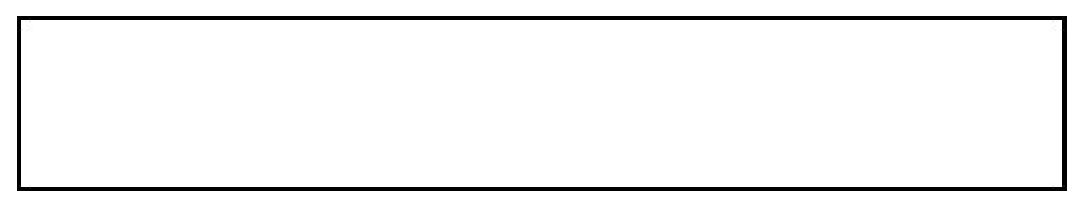
\includegraphics[width=0.9\textwidth]{fig.eps}
% \caption{This is a widefig. This is an example of long caption this is an example of long caption  this is an example of long caption this is an example of long caption}\label{fig1}
% \end{figure}

% In case of double column layout, the above format puts figure captions/images to single column width. To get spanned images, we need to provide \verb+\begin{figure*}+ \verb+...+ \verb+\end{figure*}+.

% For sample purpose, we have included the width of images in the optional argument of \verb+\includegraphics+ tag. Please ignore this. 

% \section{Algorithms, Program codes and Listings}\label{sec7}

% Packages \verb+algorithm+, \verb+algorithmicx+ and \verb+algpseudocode+ are used for setting algorithms in \LaTeX\ using the format:

% %%=============================================%%
% %% For presentation purpose, we have included  %%
% %% \bigskip command. Please ignore this.       %%
% %%=============================================%%
% \bigskip
% \begin{verbatim}
% \begin{algorithm}
% \caption{<alg-caption>}\label{<alg-label>}
% \begin{algorithmic}[1]
% . . .
% \end{algorithmic}
% \end{algorithm}
% \end{verbatim}
% \bigskip
% %%=============================================%%
% %% For presentation purpose, we have included  %%
% %% \bigskip command. Please ignore this.       %%
% %%=============================================%%

% You may refer above listed package documentations for more details before setting \verb+algorithm+ environment. For program codes, the ``verbatim'' package is required and the command to be used is \verb+\begin{verbatim}+ \verb+...+ \verb+\end{verbatim}+. 

% Similarly, for \verb+listings+, use the \verb+listings+ package. \verb+\begin{lstlisting}+ \verb+...+ \verb+\end{lstlisting}+ is used to set environments similar to \verb+verbatim+ environment. Refer to the \verb+lstlisting+ package documentation for more details.

% A fast exponentiation procedure:

% \lstset{texcl=true,basicstyle=\small\sf,commentstyle=\small\rm,mathescape=true,escapeinside={(*}{*)}}
% \begin{lstlisting}
% begin
%   for $i:=1$ to $10$ step $1$ do
%       expt($2,i$);  
%       newline() od                (*\textrm{Comments will be set flush to the right margin}*)
% where
% proc expt($x,n$) $\equiv$
%   $z:=1$;
%   do if $n=0$ then exit fi;
%      do if odd($n$) then exit fi;                 
%         comment: (*\textrm{This is a comment statement;}*)
%         $n:=n/2$; $x:=x*x$ od;
%      { $n>0$ };
%      $n:=n-1$; $z:=z*x$ od;
%   print($z$). 
% end
% \end{lstlisting}

% \begin{algorithm}
% \caption{Calculate $y = x^n$}\label{algo1}
% \begin{algorithmic}[1]
% \Require $n \geq 0 \vee x \neq 0$
% \Ensure $y = x^n$ 
% \State $y \Leftarrow 1$
% \If{$n < 0$}\label{algln2}
%         \State $X \Leftarrow 1 / x$
%         \State $N \Leftarrow -n$
% \Else
%         \State $X \Leftarrow x$
%         \State $N \Leftarrow n$
% \EndIf
% \While{$N \neq 0$}
%         \If{$N$ is even}
%             \State $X \Leftarrow X \times X$
%             \State $N \Leftarrow N / 2$
%         \Else[$N$ is odd]
%             \State $y \Leftarrow y \times X$
%             \State $N \Leftarrow N - 1$
%         \EndIf
% \EndWhile
% \end{algorithmic}
% \end{algorithm}

% %%=============================================%%
% %% For presentation purpose, we have included  %%
% %% \bigskip command. Please ignore this.       %%
% %%=============================================%%
% \bigskip
% \begin{minipage}{\hsize}%
% \lstset{frame=single,framexleftmargin=-1pt,framexrightmargin=-17pt,framesep=12pt,linewidth=0.98\textwidth,language=pascal}% Set your language (you can change the language for each code-block optionally)
% %%% Start your code-block
% \begin{lstlisting}
% for i:=maxint to 0 do
% begin
% { do nothing }
% end;
% Write('Case insensitive ');
% Write('Pascal keywords.');
% \end{lstlisting}
% \end{minipage}

% \section{Cross referencing}\label{sec8}

% Environments such as figure, table, equation and align can have a label
% declared via the \verb+\label{#label}+ command. For figures and table
% environments use the \verb+\label{}+ command inside or just
% below the \verb+\caption{}+ command. You can then use the
% \verb+\ref{#label}+ command to cross-reference them. As an example, consider
% the label declared for Figure~\ref{fig1} which is
% \verb+\label{fig1}+. To cross-reference it, use the command 
% \verb+Figure \ref{fig1}+, for which it comes up as
% ``Figure~\ref{fig1}''. 

% To reference line numbers in an algorithm, consider the label declared for the line number 2 of Algorithm~\ref{algo1} is \verb+\label{algln2}+. To cross-reference it, use the command \verb+\ref{algln2}+ for which it comes up as line~\ref{algln2} of Algorithm~\ref{algo1}.

% \subsection{Details on reference citations}\label{subsec7}

% Standard \LaTeX\ permits only numerical citations. To support both numerical and author-year citations this template uses \verb+natbib+ \LaTeX\ package. For style guidance please refer to the template user manual.

% Here is an example for \verb+\cite{...}+: \cite{bib1}. Another example for \verb+\citep{...}+: \citep{bib2}. For author-year citation mode, \verb+\cite{...}+ prints Jones et al. (1990) and \verb+\citep{...}+ prints (Jones et al., 1990).

% All cited bib entries are printed at the end of this article: \cite{bib3}, \cite{bib4}, \cite{bib5}, \cite{bib6}, \cite{bib7}, \cite{bib8}, \cite{bib9}, \cite{bib10}, \cite{bib11}, \cite{bib12} and \cite{bib13}.

% \section{Examples for theorem like environments}\label{sec10}

% For theorem like environments, we require \verb+amsthm+ package. There are three types of predefined theorem styles exists---\verb+thmstyleone+, \verb+thmstyletwo+ and \verb+thmstylethree+ 

% %%=============================================%%
% %% For presentation purpose, we have included  %%
% %% \bigskip command. Please ignore this.       %%
% %%=============================================%%
% \bigskip
% \begin{tabular}{|l|p{19pc}|}
% \hline
% \verb+thmstyleone+ & Numbered, theorem head in bold font and theorem text in italic style \\\hline
% \verb+thmstyletwo+ & Numbered, theorem head in roman font and theorem text in italic style \\\hline
% \verb+thmstylethree+ & Numbered, theorem head in bold font and theorem text in roman style \\\hline
% \end{tabular}
% \bigskip
% %%=============================================%%
% %% For presentation purpose, we have included  %%
% %% \bigskip command. Please ignore this.       %%
% %%=============================================%%

% For mathematics journals, theorem styles can be included as shown in the following examples:

% \begin{theorem}[Theorem subhead]\label{thm1}
% Example theorem text. Example theorem text. Example theorem text. Example theorem text. Example theorem text. 
% Example theorem text. Example theorem text. Example theorem text. Example theorem text. Example theorem text. 
% Example theorem text. 
% \end{theorem}

% Sample body text. Sample body text. Sample body text. Sample body text. Sample body text. Sample body text. Sample body text. Sample body text.

% \begin{proposition}
% Example proposition text. Example proposition text. Example proposition text. Example proposition text. Example proposition text. 
% Example proposition text. Example proposition text. Example proposition text. Example proposition text. Example proposition text. 
% \end{proposition}

% Sample body text. Sample body text. Sample body text. Sample body text. Sample body text. Sample body text. Sample body text. Sample body text.

% \begin{example}
% Phasellus adipiscing semper elit. Proin fermentum massa
% ac quam. Sed diam turpis, molestie vitae, placerat a, molestie nec, leo. Maecenas lacinia. Nam ipsum ligula, eleifend
% at, accumsan nec, suscipit a, ipsum. Morbi blandit ligula feugiat magna. Nunc eleifend consequat lorem. 
% \end{example}

% Sample body text. Sample body text. Sample body text. Sample body text. Sample body text. Sample body text. Sample body text. Sample body text.

% \begin{remark}
% Phasellus adipiscing semper elit. Proin fermentum massa
% ac quam. Sed diam turpis, molestie vitae, placerat a, molestie nec, leo. Maecenas lacinia. Nam ipsum ligula, eleifend
% at, accumsan nec, suscipit a, ipsum. Morbi blandit ligula feugiat magna. Nunc eleifend consequat lorem. 
% \end{remark}

% Sample body text. Sample body text. Sample body text. Sample body text. Sample body text. Sample body text. Sample body text. Sample body text.

% \begin{definition}[Definition sub head]
% Example definition text. Example definition text. Example definition text. Example definition text. Example definition text. Example definition text. Example definition text. Example definition text. 
% \end{definition}

% Additionally a predefined ``proof'' environment is available: \verb+\begin{proof}+ \verb+...+ \verb+\end{proof}+. This prints a ``Proof'' head in italic font style and the ``body text'' in roman font style with an open square at the end of each proof environment. 

% \begin{proof}
% Example for proof text. Example for proof text. Example for proof text. Example for proof text. Example for proof text. Example for proof text. Example for proof text. Example for proof text. Example for proof text. Example for proof text. 
% \end{proof}

% Sample body text. Sample body text. Sample body text. Sample body text. Sample body text. Sample body text. Sample body text. Sample body text.

% \begin{proof}[Proof of Theorem~{\upshape\ref{thm1}}]
% Example for proof text. Example for proof text. Example for proof text. Example for proof text. Example for proof text. Example for proof text. Example for proof text. Example for proof text. Example for proof text. Example for proof text. 
% \end{proof}

% \noindent
% For a quote environment, use \verb+\begin{quote}...\end{quote}+
% \begin{quote}
% Quoted text example. Aliquam porttitor quam a lacus. Praesent vel arcu ut tortor cursus volutpat. In vitae pede quis diam bibendum placerat. Fusce elementum
% convallis neque. Sed dolor orci, scelerisque ac, dapibus nec, ultricies ut, mi. Duis nec dui quis leo sagittis commodo.
% \end{quote}

% Sample body text. Sample body text. Sample body text. Sample body text. Sample body text (refer Figure~\ref{fig1}). Sample body text. Sample body text. Sample body text (refer Table~\ref{tab3}). 

% \section{Methods}\label{sec11}

% Topical subheadings are allowed. Authors must ensure that their Methods section includes adequate experimental and characterization data necessary for others in the field to reproduce their work. Authors are encouraged to include RIIDs where appropriate. 

% \textbf{Ethical approval declarations} (only required where applicable) Any article reporting experiment/s carried out on (i)~live vertebrate (or higher invertebrates), (ii)~humans or (iii)~human samples must include an unambiguous statement within the methods section that meets the following requirements: 

% \begin{enumerate}[1.]
% \item Approval: a statement which confirms that all experimental protocols were approved by a named institutional and/or licensing committee. Please identify the approving body in the methods section

% \item Accordance: a statement explicitly saying that the methods were carried out in accordance with the relevant guidelines and regulations

% \item Informed consent (for experiments involving humans or human tissue samples): include a statement confirming that informed consent was obtained from all participants and/or their legal guardian/s
% \end{enumerate}

% If your manuscript includes potentially identifying patient/participant information, or if it describes human transplantation research, or if it reports results of a clinical trial then  additional information will be required. Please visit (\url{https://www.nature.com/nature-research/editorial-policies}) for Nature Portfolio journals, (\url{https://www.springer.com/gp/authors-editors/journal-author/journal-author-helpdesk/publishing-ethics/14214}) for Springer Nature journals, or (\url{https://www.biomedcentral.com/getpublished/editorial-policies\#ethics+and+consent}) for BMC.

% \section{Discussion}\label{sec12}

% Discussions should be brief and focused. In some disciplines use of Discussion or `Conclusion' is interchangeable. It is not mandatory to use both. Some journals prefer a section `Results and Discussion' followed by a section `Conclusion'. Please refer to Journal-level guidance for any specific requirements. 

% \section{Conclusion}\label{sec13}

% Conclusions may be used to restate your hypothesis or research question, restate your major findings, explain the relevance and the added value of your work, highlight any limitations of your study, describe future directions for research and recommendations. 

% In some disciplines use of Discussion or 'Conclusion' is interchangeable. It is not mandatory to use both. Please refer to Journal-level guidance for any specific requirements. 

% \backmatter

% \bmhead{Supplementary information}

% If your article has accompanying supplementary file/s please state so here. 

% Authors reporting data from electrophoretic gels and blots should supply the full unprocessed scans for key as part of their Supplementary information. This may be requested by the editorial team/s if it is missing.

% Please refer to Journal-level guidance for any specific requirements.

\bmhead{Acknowledgements}

  Funded by the Deutsche Forschungsgemeinschaft (DFG, German Research Foundation) – Project-ID 511263698 – TRR 375.\\
  Funded by the Deutsche Forschungsgemeinschaft (DFG, German Research Foundation) – Project-ID 523648868 - FOR 5701.\\
  Calculations for this research were conducted on the Lichtenberg high performance computer of the TU Darmstadt. \\
This research was enabled by the FEniCSx library\added{~\cite{fenicsx_documentation}}, and we thank its developers and the community for their valuable contributions.\\

% Acknowledgements are not compulsory. Where included they should be brief. Grant or contribution numbers may be acknowledged.

% Please refer to Journal-level guidance for any specific requirements.

\section*{Declarations}

\bmhead{Ethical Approval} not applicable.

\bmhead{Funding} Funded by the Deutsche Forschungsgemeinschaft (DFG, German Research Foundation) – Project-ID 511263698 – TRR 375.\\
  Funded by the Deutsche Forschungsgemeinschaft (DFG, German Research Foundation) – Project-ID 523648868 - FOR 5701.\\

  \bmhead{Availability of data and materials} Research data will be published after review. The data will be published on Zenodo and referenced here in the final version of the manuscript.
% Some journals require declarations to be submitted in a standardised format. Please check the Instructions for Authors of the journal to which you are submitting to see if you need to complete this section. If yes, your manuscript must contain the following sections under the heading `Declarations':

% \begin{itemize}
% \item Funding
% \item Conflict of interest/Competing interests (check journal-specific guidelines for which heading to use)
% \item Ethics approval and consent to participate
% \item Consent for publication
% \item Data availability 
% \item Materials availability
% \item Code availability 
% \item Author contribution
% \end{itemize}

% \noindent
% If any of the sections are not relevant to your manuscript, please include the heading and write `Not applicable' for that section. 

% %%===================================================%%
% %% For presentation purpose, we have included        %%
% %% \bigskip command. Please ignore this.             %%
% %%===================================================%%
% \bigskip
% \begin{flushleft}%
% Editorial Policies for:

% \bigskip\noindent
% Springer journals and proceedings: \url{https://www.springer.com/gp/editorial-policies}

% \bigskip\noindent
% Nature Portfolio journals: \url{https://www.nature.com/nature-research/editorial-policies}

% \bigskip\noindent
% \textit{Scientific Reports}: \url{https://www.nature.com/srep/journal-policies/editorial-policies}

% \bigskip\noindent
% BMC journals: \url{https://www.biomedcentral.com/getpublished/editorial-policies}
% \end{flushleft}

% \begin{appendices}

% \section{Section title of first appendix}\label{secA1}

% An appendix contains supplementary information that is not an essential part of the text itself but which may be helpful in providing a more comprehensive understanding of the research problem or it is information that is too cumbersome to be included in the body of the paper.

% %%=============================================%%
% %% For submissions to Nature Portfolio Journals %%
% %% please use the heading ``Extended Data''.   %%
% %%=============================================%%

% %%=============================================================%%
% %% Sample for another appendix section			       %%
% %%=============================================================%%

% %% \section{Example of another appendix section}\label{secA2}%
% %% Appendices may be used for helpful, supporting or essential material that would otherwise 
% %% clutter, break up or be distracting to the text. Appendices can consist of sections, figures, 
% %% tables and equations etc.

% \end{appendices}

%%===========================================================================================%%
%% If you are submitting to one of the Nature Portfolio journals, using the eJP submission   %%
%% system, please include the references within the manuscript file itself. You may do this  %%
%% by copying the reference list from your .bbl file, paste it into the main manuscript .tex %%
%% file, and delete the associated \verb+\bibliography+ commands.                            %%
%%===========================================================================================%%

 % \bibliographystyle{sn-basic}
% \bibliography{bib/literatur.bib}% common bib file
%% if required, the content of .bbl file can be included here once bbl is generated
%%\input sn-article.bbl
% \input{./schueter_medda_mueller_klaim_2025.bbl}

\begin{thebibliography}{24}
% BibTex style file: bmc-mathphys.bst (version 2.1), 2014-07-24
\ifx \bisbn   \undefined \def \bisbn  #1{ISBN #1}\fi
\ifx \binits  \undefined \def \binits#1{#1}\fi
\ifx \bauthor  \undefined \def \bauthor#1{#1}\fi
\ifx \batitle  \undefined \def \batitle#1{#1}\fi
\ifx \bjtitle  \undefined \def \bjtitle#1{#1}\fi
\ifx \bvolume  \undefined \def \bvolume#1{\textbf{#1}}\fi
\ifx \byear  \undefined \def \byear#1{#1}\fi
\ifx \bissue  \undefined \def \bissue#1{#1}\fi
\ifx \bfpage  \undefined \def \bfpage#1{#1}\fi
\ifx \blpage  \undefined \def \blpage #1{#1}\fi
\ifx \burl  \undefined \def \burl#1{\textsf{#1}}\fi
\ifx \doiurl  \undefined \def \doiurl#1{\url{https://doi.org/#1}}\fi
\ifx \betal  \undefined \def \betal{\textit{et al.}}\fi
\ifx \binstitute  \undefined \def \binstitute#1{#1}\fi
\ifx \binstitutionaled  \undefined \def \binstitutionaled#1{#1}\fi
\ifx \bctitle  \undefined \def \bctitle#1{#1}\fi
\ifx \beditor  \undefined \def \beditor#1{#1}\fi
\ifx \bpublisher  \undefined \def \bpublisher#1{#1}\fi
\ifx \bbtitle  \undefined \def \bbtitle#1{#1}\fi
\ifx \bedition  \undefined \def \bedition#1{#1}\fi
\ifx \bseriesno  \undefined \def \bseriesno#1{#1}\fi
\ifx \blocation  \undefined \def \blocation#1{#1}\fi
\ifx \bsertitle  \undefined \def \bsertitle#1{#1}\fi
\ifx \bsnm \undefined \def \bsnm#1{#1}\fi
\ifx \bsuffix \undefined \def \bsuffix#1{#1}\fi
\ifx \bparticle \undefined \def \bparticle#1{#1}\fi
\ifx \barticle \undefined \def \barticle#1{#1}\fi
\bibcommenthead
\ifx \bconfdate \undefined \def \bconfdate #1{#1}\fi
\ifx \botherref \undefined \def \botherref #1{#1}\fi
\ifx \url \undefined \def \url#1{\textsf{#1}}\fi
\ifx \bchapter \undefined \def \bchapter#1{#1}\fi
\ifx \bbook \undefined \def \bbook#1{#1}\fi
\ifx \bcomment \undefined \def \bcomment#1{#1}\fi
\ifx \oauthor \undefined \def \oauthor#1{#1}\fi
\ifx \citeauthoryear \undefined \def \citeauthoryear#1{#1}\fi
\ifx \endbibitem  \undefined \def \endbibitem {}\fi
\ifx \bconflocation  \undefined \def \bconflocation#1{#1}\fi
\ifx \arxivurl  \undefined \def \arxivurl#1{\textsf{#1}}\fi
\csname PreBibitemsHook\endcsname

%%% 1
\bibitem[\protect\citeauthoryear{Hossain et~al.}{2014}]{hossain_effective_2014}
\begin{barticle}
\bauthor{\bsnm{Hossain}, \binits{M.Z.}},
\bauthor{\bsnm{Hsueh}, \binits{C.-J.}},
\bauthor{\bsnm{Bourdin}, \binits{B.}},
\bauthor{\bsnm{Bhattacharya}, \binits{K.}}:
\batitle{Effective toughness of heterogeneous media}.
\bjtitle{Journal of the Mechanics and Physics of Solids}
\bvolume{71},
\bfpage{15}--\blpage{32}
(\byear{2014})
\doiurl{10.1016/j.jmps.2014.06.002}
\end{barticle}
\endbibitem

%%% 2
\bibitem[\protect\citeauthoryear{Gross and Seelig}{2011}]{gross_fracture_2011}
\begin{bbook}
\bauthor{\bsnm{Gross}, \binits{D.}},
\bauthor{\bsnm{Seelig}, \binits{T.}}:
\bbtitle{Fracture {{Mechanics}}: {{With}} an {{Introduction}} to {{Micromechanics}}}.
\bsertitle{Mechanical {{Engineering Series}}}.
\bpublisher{Springer},
\blocation{Berlin, Heidelberg}
(\byear{2011}).
\doiurl{10.1007/978-3-642-19240-1}
\end{bbook}
\endbibitem

%%% 3
\bibitem[\protect\citeauthoryear{Hauser et~al.}{2021}]{hauser_porosity_2021}
\begin{barticle}
\bauthor{\bsnm{Hauser}, \binits{T.}},
\bauthor{\bsnm{Reisch}, \binits{R.T.}},
\bauthor{\bsnm{Breese}, \binits{P.P.}},
\bauthor{\bsnm{Lutz}, \binits{B.S.}},
\bauthor{\bsnm{Pantano}, \binits{M.}},
\bauthor{\bsnm{Nalam}, \binits{Y.}},
\bauthor{\bsnm{Bela}, \binits{K.}},
\bauthor{\bsnm{Kamps}, \binits{T.}},
\bauthor{\bsnm{Volpp}, \binits{J.}},
\bauthor{\bsnm{Kaplan}, \binits{A.F.H.}}:
\batitle{Porosity in wire arc additive manufacturing of aluminium alloys}.
\bjtitle{Additive Manufacturing}
\bvolume{41},
\bfpage{101993}
(\byear{2021})
\doiurl{10.1016/j.addma.2021.101993}
\end{barticle}
\endbibitem

%%% 4
\bibitem[\protect\citeauthoryear{Lebihain}{2021}]{lebihain_brittle_2021}
\begin{barticle}
\bauthor{\bsnm{Lebihain}, \binits{M.}}:
\batitle{Towards brittle materials with tailored fracture properties: The decisive influence of the material disorder and its microstructure}.
\bjtitle{International Journal of Fracture}
\bvolume{230}(\bissue{1-2}),
\bfpage{99}
(\byear{2021})
\doiurl{10.1007/s10704-021-00538-7}
\end{barticle}
\endbibitem

%%% 5
\bibitem[\protect\citeauthoryear{Schneider}{2020}]{schneider_fftbased_2020}
\begin{barticle}
\bauthor{\bsnm{Schneider}, \binits{M.}}:
\batitle{An {{FFT-based}} method for computing weighted minimal surfaces in microstructures with applications to the computational homogenization of brittle fracture}.
\bjtitle{International Journal for Numerical Methods in Engineering}
\bvolume{121}(\bissue{7}),
\bfpage{1367}--\blpage{1387}
(\byear{2020})
\doiurl{10.1002/nme.6270}
\end{barticle}
\endbibitem

%%% 6
\bibitem[\protect\citeauthoryear{Bourdin et~al.}{2008}]{bourdin_variational_2008}
\begin{barticle}
\bauthor{\bsnm{Bourdin}, \binits{B.}},
\bauthor{\bsnm{Francfort}, \binits{G.A.}},
\bauthor{\bsnm{Marigo}, \binits{J.-J.}}:
\batitle{The {{Variational Approach}} to {{Fracture}}}.
\bjtitle{Journal of Elasticity}
\bvolume{91}(\bissue{1}),
\bfpage{5}--\blpage{148}
(\byear{2008})
\doiurl{10.1007/s10659-007-9107-3}
\end{barticle}
\endbibitem

%%% 7
\bibitem[\protect\citeauthoryear{Ernesti and Schneider}{2021}]{ernesti_fast_2021}
\begin{barticle}
\bauthor{\bsnm{Ernesti}, \binits{F.}},
\bauthor{\bsnm{Schneider}, \binits{M.}}:
\batitle{A fast {{Fourier}} transform based method for computing the effective crack energy of a heterogeneous material on a combinatorially consistent grid}.
\bjtitle{International Journal for Numerical Methods in Engineering}
\bvolume{122}(\bissue{21}),
\bfpage{6283}--\blpage{6307}
(\byear{2021})
\doiurl{10.1002/nme.6792}
\end{barticle}
\endbibitem

%%% 8
\bibitem[\protect\citeauthoryear{Ernesti and Schneider}{2022}]{ernesti_computing_2022}
\begin{barticle}
\bauthor{\bsnm{Ernesti}, \binits{F.}},
\bauthor{\bsnm{Schneider}, \binits{M.}}:
\batitle{Computing the effective crack energy of heterogeneous and anisotropic microstructures via anisotropic minimal surfaces}.
\bjtitle{Computational Mechanics}
\bvolume{69}(\bissue{1}),
\bfpage{45}--\blpage{57}
(\byear{2022})
\doiurl{10.1007/s00466-021-02082-6}
\end{barticle}
\endbibitem

%%% 9
\bibitem[\protect\citeauthoryear{Michel and Suquet}{2022}]{michel_merits_2022}
\begin{barticle}
\bauthor{\bsnm{Michel}, \binits{J.-C.}},
\bauthor{\bsnm{Suquet}, \binits{P.}}:
\batitle{Merits and limits of a variational definition of the effective toughness of heterogeneous materials}.
\bjtitle{Journal of the Mechanics and Physics of Solids}
\bvolume{164},
\bfpage{104889}
(\byear{2022})
\doiurl{10.1016/j.jmps.2022.104889}
\end{barticle}
\endbibitem

%%% 10
\bibitem[\protect\citeauthoryear{Hsueh et~al.}{2018}]{hsueh_stress_2018}
\begin{barticle}
\bauthor{\bsnm{Hsueh}, \binits{C.-J.}},
\bauthor{\bsnm{Avellar}, \binits{L.}},
\bauthor{\bsnm{Bourdin}, \binits{B.}},
\bauthor{\bsnm{Ravichandran}, \binits{G.}},
\bauthor{\bsnm{Bhattacharya}, \binits{K.}}:
\batitle{Stress fluctuation, crack renucleation and toughening in layered materials}.
\bjtitle{Journal of the Mechanics and Physics of Solids}
\bvolume{120},
\bfpage{68}--\blpage{78}
(\byear{2018})
\doiurl{10.1016/j.jmps.2018.04.011}
\end{barticle}
\endbibitem

%%% 11
\bibitem[\protect\citeauthoryear{Brach et~al.}{2019}]{brach_anisotropy_2019}
\begin{barticle}
\bauthor{\bsnm{Brach}, \binits{S.}},
\bauthor{\bsnm{Hossain}, \binits{M.Z.}},
\bauthor{\bsnm{Bourdin}, \binits{B.}},
\bauthor{\bsnm{Bhattacharya}, \binits{K.}}:
\batitle{Anisotropy of the effective toughness of layered media}.
\bjtitle{Journal of the Mechanics and Physics of Solids}
\bvolume{131},
\bfpage{96}--\blpage{111}
(\byear{2019})
\doiurl{10.1016/j.jmps.2019.06.021}
\end{barticle}
\endbibitem

%%% 12
\bibitem[\protect\citeauthoryear{Ambati et~al.}{2015}]{ambati_review_2015}
\begin{barticle}
\bauthor{\bsnm{Ambati}, \binits{M.}},
\bauthor{\bsnm{Gerasimov}, \binits{T.}},
\bauthor{\bsnm{De~Lorenzis}, \binits{L.}}:
\batitle{A review on phase-field models of brittle fracture and a new fast hybrid formulation}.
\bjtitle{Computational Mechanics}
\bvolume{55}(\bissue{2}),
\bfpage{383}--\blpage{405}
(\byear{2015})
\doiurl{10.1007/s00466-014-1109-y}
\end{barticle}
\endbibitem

%%% 13
\bibitem[\protect\citeauthoryear{Schl{\"u}ter and M{\"u}ller}{2025a}]{schlueter_ermittlung_2025}
\begin{botherref}
\oauthor{\bsnm{Schl{\"u}ter}, \binits{A.}},
\oauthor{\bsnm{M{\"u}ller}, \binits{R.}}:
{Ermittlung des effektiven Risswiderstands in por\"osen Materialien\dots}.
https://dvm-wissen.de/de/57-tagung-des-dvm-arbeitskreises-bruchmechanik-und-bauteilsicherheit-/478-BR-2025-472.html?sp=undefined\&q=Kategorien-Bruchmechanik+und+Bauteilsicherheit
(2025)
\end{botherref}
\endbibitem

%%% 14
\bibitem[\protect\citeauthoryear{Schl{\"u}ter and M{\"u}ller}{2025b}]{schluter_determination_2025}
\begin{barticle}
\bauthor{\bsnm{Schl{\"u}ter}, \binits{A.}},
\bauthor{\bsnm{M{\"u}ller}, \binits{R.}}:
\batitle{Determination of the effective crack resistance in porous materials using a fracture phase-field model}.
\bjtitle{Engineering Fracture Mechanics}
\bvolume{326},
\bfpage{111348}
(\byear{2025})
\doiurl{10.1016/j.engfracmech.2025.111348}
\end{barticle}
\endbibitem

%%% 15
\bibitem[\protect\citeauthoryear{Schl{\"u}ter et~al.}{2025}]{schluter_influence_2025}
\begin{barticle}
\bauthor{\bsnm{Schl{\"u}ter}, \binits{A.}},
\bauthor{\bsnm{Medda}, \binits{R.}},
\bauthor{\bsnm{M{\"u}ller}, \binits{R.}}:
\batitle{Influence of {{Material Nonlinearity}} on the {{Effective Fracture Resistance}} of {{Porous Materials}}}.
\bjtitle{PAMM}
\bvolume{25}(\bissue{4}),
\bfpage{70044}
(\byear{2025})
\doiurl{10.1002/pamm.70044}
\end{barticle}
\endbibitem

%%% 16
\bibitem[\protect\citeauthoryear{{Nemat-Nasser} and Hori}{2013}]{nemat-nasser_micromechanics_2013}
\begin{bbook}
\bauthor{\bsnm{{Nemat-Nasser}}, \binits{S.}},
\bauthor{\bsnm{Hori}, \binits{M.}}:
\bbtitle{Micromechanics: Overall Properties of Heterogeneous Materials}.
\bpublisher{Elsevier}, \blocation{???}
(\byear{2013})
\end{bbook}
\endbibitem

%%% 17
\bibitem[\protect\citeauthoryear{Bohnen et~al.}{2024}]{bohnen_simulation_2024}
\begin{bchapter}
\bauthor{\bsnm{Bohnen}, \binits{M.}},
\bauthor{\bsnm{M{\"u}ller}, \binits{R.}},
\bauthor{\bsnm{Gross}, \binits{D.}}:
\bctitle{Simulation of~{{Crack Propagation}} in~{{Heterogeneous Materials}} by~a~{{Fracture Phase Field}}}.
In: \beditor{\bsnm{M{\"u}ller}, \binits{W.H.}},
\beditor{\bsnm{Noe}, \binits{A.}},
\beditor{\bsnm{Ferber}, \binits{F.}} (eds.)
\bbtitle{New {{Achievements}} in {{Mechanics}}: {{A Tribute}} to {{Klaus Peter Herrmann}}},
pp. \bfpage{191}--\blpage{215}.
\bpublisher{Springer},
\blocation{Cham}
(\byear{2024}).
\doiurl{10.1007/978-3-031-56132-0_10}
\end{bchapter}
\endbibitem

%%% 18
\bibitem[\protect\citeauthoryear{Noll et~al.}{2020}]{noll_3d_2020}
\begin{barticle}
\bauthor{\bsnm{Noll}, \binits{T.}},
\bauthor{\bsnm{Kuhn}, \binits{C.}},
\bauthor{\bsnm{Olesch}, \binits{D.}},
\bauthor{\bsnm{M{\"u}ller}, \binits{R.}}:
\batitle{{{3D}} phase field simulations of ductile fracture}.
\bjtitle{GAMM-Mitteilungen}
\bvolume{43}(\bissue{2}),
\bfpage{202000008}
(\byear{2020})
\doiurl{10.1002/gamm.202000008}
\end{barticle}
\endbibitem

%%% 19
\bibitem[\protect\citeauthoryear{Chambolle}{2004}]{chambolle_approximation_2004}
\begin{barticle}
\bauthor{\bsnm{Chambolle}, \binits{A.}}:
\batitle{An approximation result for special functions with bounded deformation}.
\bjtitle{Journal de Math\'ematiques Pures et Appliqu\'ees}
\bvolume{83}(\bissue{7}),
\bfpage{929}--\blpage{954}
(\byear{2004})
\doiurl{10.1016/j.matpur.2004.02.004}
\end{barticle}
\endbibitem

%%% 20
\bibitem[\protect\citeauthoryear{Kuhn and M{\"u}ller}{2010}]{kuhn_continuum_2010}
\begin{barticle}
\bauthor{\bsnm{Kuhn}, \binits{C.}},
\bauthor{\bsnm{M{\"u}ller}, \binits{R.}}:
\batitle{A continuum phase field model for fracture}.
\bjtitle{Engineering Fracture Mechanics}
\bvolume{77}(\bissue{18}),
\bfpage{3625}--\blpage{3634}
(\byear{2010})
\doiurl{10.1016/j.engfracmech.2010.08.009}
\end{barticle}
\endbibitem

%%% 21
\bibitem[\protect\citeauthoryear{Tann{\'e} et~al.}{2018}]{tanne_crack_2018}
\begin{barticle}
\bauthor{\bsnm{Tann{\'e}}, \binits{E.}},
\bauthor{\bsnm{Li}, \binits{T.}},
\bauthor{\bsnm{Bourdin}, \binits{B.}},
\bauthor{\bsnm{Marigo}, \binits{J.-J.}},
\bauthor{\bsnm{Maurini}, \binits{C.}}:
\batitle{Crack nucleation in variational phase-field models of brittle fracture}.
\bjtitle{Journal of the Mechanics and Physics of Solids}
\bvolume{110},
\bfpage{80}--\blpage{99}
(\byear{2018})
\doiurl{10.1016/j.jmps.2017.09.006}
\end{barticle}
\endbibitem

%%% 22
\bibitem[\protect\citeauthoryear{Schlueter}{2018}]{schlueter_phase_2018}
\begin{botherref}
\oauthor{\bsnm{Schlueter}, \binits{A.}}:
Phase {{Field Modeling}} of {{Dynamic Brittle Fracture}}.
PhD thesis,
Technische Universit\"at Kaiserslautern
(June 2018)
\end{botherref}
\endbibitem

%%% 23
\bibitem[\protect\citeauthoryear{Kuhn}{2013}]{kuhn_numerical_2013}
\begin{botherref}
\oauthor{\bsnm{Kuhn}, \binits{C.}}:
Numerical and {{Analytical Investigation}} of a {{Phase Field Model}} for {{Fracture}}.
PhD thesis,
Technische Universit\"at Kaiserslautern
(March 2013)
\end{botherref}
\endbibitem

%%% 24
\bibitem[\protect\citeauthoryear{{FEniCS Project}}{{FEniCS Project}}{2025}]{fenicsx_documentation}
\begin{botherref}
\oauthor{\bsnm{{FEniCS Project}}}:
FEniCSx Documentation.
\url{https://fenicsproject.org/}.
Accessed 22 July 2025
\end{botherref}
\endbibitem

\end{thebibliography}

\end{document}
